\documentclass{article}

% Packages, verbatim style, and title block.
% Loaded by main.tex; do not put \documentclass or \begin{document} here.

% NeurIPS 2024 style: US letter, 5.5in x 9in text block, 10pt Times, title between
% rules. [preprint] prints the authors (the default mode anonymises them and adds
% line numbers); [nonatbib] keeps the numeric IEEEtran references.
\usepackage[preprint,nonatbib]{neurips_2024}

% Language and fonts. T5 must be the last (default) encoding so that Vietnamese
% IRIs and labels (Nguyễn_Công_Phượng, Thể_loại:…) typeset with pdflatex.
% neurips_2024 asks for Times (ptm) and Helvetica (phv), which have no T5 glyphs;
% TeX Gyre Termes and Heros are the same designs with T5 support. Latin Modern
% stays as the typewriter font for IRIs and code.
\usepackage[utf8]{inputenc}
\usepackage[T1,T5]{fontenc}
\usepackage{lmodern}
\usepackage{tgtermes}
\usepackage{tgheros}
\usepackage[vietnamese,english]{babel}

% Useful packages
\usepackage{amsmath, amssymb}
\usepackage{graphicx}
\usepackage{adjustbox}
\usepackage{xcolor}
\usepackage{float}
\usepackage[font=small,labelfont=bf]{caption}
\usepackage{subcaption}
\usepackage{microtype}

\usepackage{booktabs}
\usepackage{multirow}
\usepackage{tabularx}
\usepackage{array}

% Verbatim blocks (SPARQL, Turtle, curl). listings cannot handle UTF-8
% Vietnamese characters, fancyvrb passes them through to the T5 font.
% neurips_2024 makes \footnotesize 9pt; 8pt keeps the longest lines (~95
% characters) inside the 5.5in text block. samepage keeps a block on one page.
\usepackage{fancyvrb}
\fvset{fontsize=\fontsize{8pt}{9.5pt}\selectfont, samepage=true, frame=single,
       framesep=1.5mm, rulecolor=\color{gray!60}}
% Floating listings keep a verbatim block on one page: \begin{listing}…\caption{…}\end{listing}
\newfloat{listing}{t}{lol}
\floatname{listing}{Listing}

% "approximately" tilde. \sim is a mathrel, so bare $\sim$5 gets thick
% relation spacing on both sides; \mathord strips it.
\newcommand{\apx}{\ensuremath{\mathord{\sim}}}

% Vocabulary terms and IRIs in running text: \term{vio:playedFor}.
% Typewriter fonts do not hyphenate by default; long IRIs would overrun the
% margin, so allow hyphenation in \term and give paragraphs extra stretch.
\newcommand{\term}[1]{\text{\ttfamily\hyphenchar\font=45\relax #1}}
\setlength{\emergencystretch}{3em}

% Placeholder the group must fill in before submission (prints in red).
\newcommand{\fillin}[1]{\textcolor{red}{[#1]}}

% --- TikZ for schematic figures ---
\usepackage{tikz}
\usetikzlibrary{arrows.meta, calc, positioning, backgrounds, shapes.geometric}
% Accent colours: project vocabulary (blue), inferred triples (orange),
% external datasets and asserted edges (gray).
\definecolor{accblue}{HTML}{2A78D6}
\definecolor{accorange}{HTML}{EB6834}
\definecolor{accgray}{HTML}{8A8984}
% RDFS graph figure (figures/rdfs_graph.tex): instance nodes, property nodes and
% domain/range edges, entailed triples
\colorlet{rdfsdraw}{accblue}
\colorlet{rdfsfill}{accblue!6}
\colorlet{rdfsprop}{accblue!75!black}
\colorlet{rdfsaxiom}{accorange}

\usepackage[colorlinks=true, allcolors=blue]{hyperref}

\title{Building a Vietnamese DBpedia:\\ Linked Open Data from Vietnamese Wikipedia}

% NeurIPS author block: \And separates authors on one line; the first line of
% each block is bold, the next lines are the student ID.
\author{%
  Ha Thi Kim Phung \\ 20242460M
  \And
  Do Ngoc Trung \\ 20232311M
  \And
  Bui Duc Phan Hoang \\ 20252004M
  \And
  Do Hoang Dung \\ 20241184M
}

% Footnote at the bottom of page 1, where NeurIPS prints the conference notice.
\makeatletter
\renewcommand{\@noticestring}{%
  Semantic Web course project, Topic~2: \emph{Build a DBpedia version for Vietnamese language}.
  Group~23, lecturer Dr.~Do Ba Lam. Hanoi University of Science and Technology, October 2026.%
}
\makeatother


\graphicspath{{figures/}}

\begin{document}
\maketitle

% =========================
% =========================
\begin{abstract}
DBpedia turns the semi-structured content of Wikipedia into Linked Data that
can be queried with SPARQL and joined with other datasets. This report
describes a DBpedia-style knowledge base for Vietnamese built from Vietnamese
Wikipedia and Wikidata for a closed but densely connected domain: Vietnamese
football (players, clubs, national teams and stadiums), provinces and
universities. We (i)~define an OWL ontology, \term{vio:}, with 18 classes and
54 properties, each class aligned to a DBpedia Ontology ancestor; (ii)~select
990 entities through the Wikidata Query Service and collect their Vietnamese
articles through the MediaWiki API; (iii)~transform abstracts, infoboxes,
categories and redirects into 88{,}898 RDF triples with stable IRIs that the
project server dereferences, validated by eight quality checks and expanded by OWL~2~RL reasoning to
131{,}543 triples; (iv)~link 777 entities to English DBpedia and all 990 to
Wikidata with \term{owl:sameAs}, described as VoID linksets; and (v)~serve the
data through a SPARQL~1.1 Protocol endpoint, a command-line query client and a
web application with a SPARQL editor, DBpedia-style entity pages, HTTP
content negotiation and question answering in which a large language model
writes the SPARQL query and each step is shown. Reasoning lets the data be queried with
the DBpedia vocabulary (0 asserted \term{dbo:Person} instances become 659) and
answers multi-hop questions such as ``which clubs has a player played for''
through a property chain. Checked against the live DBpedia endpoint, 733 of
the 777 English links resolve to an article. The code, data and 152 automated
tests are available at
\url{https://github.com/PhungHaThiKim/vietnamese-dbpedia}.
\end{abstract}

\noindent\textbf{Key words:} DBpedia; Linked Open Data; Vietnamese Wikipedia;
ontology; OWL~2~RL; SPARQL; Wikidata; knowledge graph question answering


% =========================
\section{Introduction}

DBpedia extracts structured information from Wikipedia---infobox fields,
abstracts, categories, redirects and links between articles---and publishes it
as RDF, so that the content of an encyclopedia can be queried with SPARQL and
joined with other datasets~\cite{auer2007dbpedia, lehmann2015dbpedia}. The
English edition sits at the centre of the Linked Open Data cloud, and language
chapters publish the same kind of data for other Wikipedia
editions~\cite{kontokostas2012greek}. Vietnamese Wikipedia articles carry the
same semi-structured information: the infobox of a footballer lists his date of
birth, birthplace and every club he played for, season by season, but as
wikitext it cannot be queried. A question such as \emph{``Which players born in
Nghệ An have played for the national team, and for which club do they play
now?''} requires reading and joining several articles by hand.

This project addresses Topic~2 of the course, \emph{Build a DBpedia version for
Vietnamese language}, which consists of five tasks: (1)~define an ontology;
(2)~collect Vietnamese articles from Wikipedia; (3)~transform the data into
4-star Linked Data; (4)~establish links to the English DBpedia; and
(5)~provide an interface to query the data through a SPARQL endpoint or
terminal.

Rather than extracting all of Vietnamese Wikipedia shallowly, we extracted a
closed domain in depth: Vietnamese \emph{football} (players, clubs, national
teams, stadiums), \emph{provinces} and \emph{universities}. Its entities refer
to one another, so the graph supports multi-hop questions: player
$\rightarrow$ career station $\rightarrow$ club $\rightarrow$ home stadium
$\rightarrow$ province, player $\rightarrow$ birth province, university
$\rightarrow$ province. 777 of the 990 selected entities (78\%) have an English
Wikipedia article to link to, and 956 of the 990 articles (97\%) contain an
infobox, the main source that DBpedia extracts. Entities are selected through
Wikidata rather than through the category tree of Vietnamese Wikipedia, whose
categories editors assign inconsistently.

The contributions of this work are:
\begin{itemize}
  \item an OWL ontology, \term{vio:}, with 18 classes and 54 properties, aligned
        to the DBpedia Ontology for OWL~2~RL reasoning (Section~\ref{sec:ontology});
  \item a reproducible pipeline whose raw downloads are committed, so the
        dataset rebuilds offline (Sections~\ref{sec:collection}--\ref{sec:postprocess});
  \item 131{,}543 triples (88{,}898 asserted, 41{,}730 inferred) that pass eight
        quality checks with no error or warning (Section~\ref{sec:evaluation});
  \item 777 \term{owl:sameAs} links to English DBpedia, verified on the live
        endpoint, and 990 to Wikidata (Sections~\ref{sec:interlinking} and~\ref{sec:links});
  \item a server with a SPARQL~1.1 Protocol endpoint, IRIs dereferenced with 303
        and content negotiation, a terminal client, and a web interface with
        entity pages, an ontology browser, a SPARQL editor and step-by-step
        question answering (Section~\ref{sec:publishing}).
\end{itemize}

Table~\ref{tab:requirements} maps each task to its implementation; the following
sections cover background, design, publishing, evaluation and discussion.

\begin{table}[t]
\centering
\caption{Where each task of the assignment is implemented. Paths are under
\term{vidbpedia/}, except \term{ui/}.}
\label{tab:requirements}
\small
\begin{tabularx}{\textwidth}{@{}l>{\raggedright\arraybackslash}X>{\raggedright\arraybackslash}Xl@{}}
\toprule
Task & Implementation & Output & Section \\
\midrule
1. Ontology & \term{ontology/*.ttl}, merged by \term{kg/ontology.py}
  & 18 classes, 54 properties, 859 triples & \ref{sec:ontology} \\
2. Collect articles & \term{crawl/wikidata\_seeds.py}, \term{crawl/wiki\_enrich.py}
  & 990 entities with their Vietnamese articles & \ref{sec:collection} \\
3. 4-star data & \term{crawl/build\_rdf.py}, \term{kg/postprocess.py}
  & 131{,}543 triples in Turtle and N-Triples & \ref{sec:transform}, \ref{sec:postprocess} \\
4. Link to DBpedia & enwiki sitelinks of the Wikidata item
  & 777 \term{owl:sameAs dbr:} links, VoID linksets & \ref{sec:interlinking} \\
5. Query interface & \term{web/}: endpoint, Linked Data, Gradio; \term{ui/}: React; \term{kg/query.py}
  & \term{/sparql} endpoint, \term{query} command, Linked Data routes, web interface
  & \ref{sec:endpoint}, \ref{sec:deref}, \ref{sec:ui} \\
\bottomrule
\end{tabularx}
\end{table}

\section{Background and Related Work}
\label{sec:related}

\paragraph{DBpedia.} DBpedia~\cite{auer2007dbpedia, lehmann2015dbpedia} extracts
labels, abstracts, page identifiers, images, categories, redirects, external
links, coordinates and infobox data from every Wikipedia article. Infobox data
is published raw, as properties of the generic \term{dbp:} namespace, and
mapping-based, through community mappings to the hand-built DBpedia Ontology
(\term{dbo:}), which is cleaner but covers less. Resources are named after
their article titles, and language chapters publish their own edition under
their own namespace with links to the English one. Kontokostas et
al.~\cite{kontokostas2012greek} describe what this raises for the Greek
chapter: IRIs in a non-Latin script, language-specific templates and links
across editions. We follow this model for Vietnamese, with a small ontology
where DBpedia lacks the terms we need.

\paragraph{Linked Data.} The Linked Data principles ask for HTTP URIs that return
RDF when looked up and link to other
URIs~\cite{bernerslee2006linked, heath2011linked}. The five-star scheme grades
open data, and Tasks~3 and~4 correspond to its fourth and fifth stars. We serve
the data with \emph{303 See Other} redirects and content
negotiation~\cite{sauermann2008cooluris, hyland2014bestpractices}, describe it
with VoID~\cite{alexander2011void}, and use RDF~1.1~\cite{cyganiak2014rdf} and
SPARQL~1.1~\cite{harris2013sparql}.

\paragraph{Wikidata.} Wikidata~\cite{vrandecic2014wikidata} items carry typed
statements with qualifiers and \emph{sitelinks} to the article about them in
every Wikipedia edition, and the Wikidata Query Service exposes them through
SPARQL~\cite{malyshev2018wdqs}. We use it to select the entities, to obtain
precise dates and quantities, and, through English sitelinks, to link to DBpedia.

\paragraph{Ontology engineering and question answering.} The ontology was
designed from \emph{competency questions}, written before the schema and later
used as tests~\cite{gruninger1995methodology}. DBpedia types and shortcut
relations are derived with the OWL~2~RL profile~\cite{motik2012owl2profiles},
whose rules run by forward chaining in polynomial time, so the derived triples
can be materialised. Retrieval-augmented generation grounds the answer of a
language model in retrieved evidence~\cite{lewis2020rag}; over a knowledge
graph the retrieval can be a SPARQL query written by the model, as on our
question-answering page (Section~\ref{sec:qa}).

\section{System Design}
\label{sec:design}

\subsection{Architecture}
\label{sec:architecture}

The system is a Python package, \term{vidbpedia}, organised in four layers
(Figure~\ref{fig:architecture}). Each step is one command,
\term{python -m vidbpedia <step>}: \term{seeds}, \term{enrich},
\term{ontology}, \term{build}, \term{postprocess} and \term{serve}, plus
\term{query} for SPARQL from the terminal. Only the collection layer uses the
network: HTTP responses are cached in SQLite and the raw downloads are
committed under \term{data/raw/}, so the later layers rebuild the dataset
offline and identically. Graphs are built with the rdflib API~\cite{rdflib}
rather than by concatenating Turtle strings, which rules out syntax and
escaping errors, and a single function creates every resource IRI, so an
entity cannot receive two IRIs.

\begin{figure}[t]
\centering
\begin{adjustbox}{max width=\textwidth}
\begin{tikzpicture}[
    font=\scriptsize, >={Stealth[length=1.8mm]},
    box/.style={draw=accgray, rounded corners=2pt, align=center, text width=2.7cm,
                minimum height=1.3cm, inner sep=3pt},
    stage/.style={box, draw=accblue, fill=accblue!7},
    store/.style={box, fill=accgray!12},
    ext/.style={box, dashed},
    flow/.style={->, accgray, thick},
  ]
  \node[ext]                        (src)   {Wikidata Query Service\\[1pt] MediaWiki API\\ (vi.wikipedia.org)};
  \node[stage, right=0.45cm of src]   (crawl) {\textbf{(1) Collection}\\[1pt] \texttt{seeds}, \texttt{enrich}\\ SQLite HTTP cache};
  \node[store, right=0.45cm of crawl] (raw)   {\texttt{data/raw/} (committed)\\[1pt] Wikidata facts,\\ article metadata, infoboxes};
  \node[stage, right=0.45cm of raw]   (build) {\textbf{(2) Semantics}\\[1pt] \texttt{ontology}: merge modules\\ \texttt{build}: infobox $\rightarrow$ RDF};
  \node[stage, below=0.75cm of build] (post)  {\textbf{(3) Post-processing}\\[1pt] validate $\rightarrow$ OWL\,2\,RL\\ $\rightarrow$ VoID $\rightarrow$ export};
  \node[store, left=0.45cm of post]   (out)   {\texttt{data/}\\[1pt] 131{,}543 triples (.ttl, .nt)\\ ontology, asserted\\ and inferred parts};
  \node[stage, left=0.45cm of out]    (srv)   {\textbf{(4) Server}\\[1pt] FastAPI + React UI\\ in-memory rdflib graph\\ \texttt{/sparql} endpoint};
  \node[ext, left=0.45cm of srv]      (users) {Browsers, terminal,\\ SPARQL and RDF clients\\[1pt] LLM (OpenAI-compatible\\ API, optional)};
  \draw[flow] (src) -- (crawl);
  \draw[flow] (crawl) -- (raw);
  \draw[flow] (raw) -- (build);
  \draw[flow] (build) -- node[right, font=\tiny, text=accgray] {\texttt{data/raw/rdf/*.ttl}} (post);
  \draw[flow] (post) -- (out);
  \draw[flow] (out) -- (srv);
  \draw[flow, <->] (srv) -- (users);
\end{tikzpicture}
\end{adjustbox}
\caption{Architecture. Blue boxes are the four layers of the \texttt{vidbpedia}
package (the interface of layer~(4) is in \texttt{ui/}), gray boxes are files on
disk, dashed boxes are external systems. Only layer~(1) calls the network.}
\label{fig:architecture}
\end{figure}

% =========================================================================
\subsection{Ontology}
\label{sec:ontology}

The ontology is written as ten Turtle modules in \term{ontology/}, from
\term{000-prefixes.ttl} to \term{420-football.ttl}. They are merged in numeric order into
\term{vi-ontology.ttl} (859 triples) and checked by rdflib when merged.
Table~\ref{tab:namespaces} lists the namespaces. Following
DBpedia~\cite{lehmann2015dbpedia}, resources are named by their article title,
infobox parameters have a raw namespace, and categories are SKOS concepts.

\begin{table}[t]
\centering
\caption{Namespaces. The \texttt{vi.dbpedia.org} namespaces mirror the IRI
scheme of DBpedia language chapters.}
\label{tab:namespaces}
\small
\begin{tabularx}{\textwidth}{@{}ll>{\raggedright\arraybackslash}X@{}}
\toprule
Prefix & Namespace & Used for \\
\midrule
\term{vio:}  & \term{http://vi.dbpedia.org/ontology/} & classes and properties of this project \\
\term{vres:} & \term{http://vi.dbpedia.org/resource/} & resources (entities) \\
\term{vip:}  & \term{http://vi.dbpedia.org/property/} & raw infobox properties, like \term{dbp:} \\
\term{vcat:} & \term{http://vi.dbpedia.org/resource/Thể\_loại:} & Wikipedia categories \\
\term{dbo:}  & \term{http://dbpedia.org/ontology/} & DBpedia Ontology \\
\term{dbr:}  & \term{http://dbpedia.org/resource/} & English DBpedia resources \\
\term{wd:}   & \term{http://www.wikidata.org/entity/} & Wikidata items \\
\bottomrule
\end{tabularx}
\end{table}

\paragraph{Classes.} The ontology has two layers~\cite{heath2011linked}. The
upper layer reuses the DBpedia Ontology: \term{050-dbo-alignment.ttl} declares
the 24 DBpedia classes and 44 properties that \term{vio:} maps to, with
DBpedia's English labels, our Vietnamese labels (\term{dbo:Animal} is ``Động
vật'') and \term{rdfs:isDefinedBy dbo:}, but not DBpedia's domains and ranges.
The lower layer has 18 \term{vio:} classes in four disjoint trees: people,
organisations, locations and career stations (Table~\ref{tab:classes}). A
\term{vio:} class exists only where an axiom or a competency
question~\cite{gruninger1995methodology} needs it, such as
\term{vio:FormerProvince}; there is no \term{vio:Animal}. Each class is an
\term{rdfs:subClassOf}, not an \term{owl:equivalentClass}, of a DBpedia class,
directly or through its parent. Data described with \term{vio:} can thus be
queried with \term{dbo:} after reasoning (Section~\ref{sec:reasoning}), while
our domains, functional properties and disjointness axioms constrain only our
own data, avoiding the Exclusivity anti-pattern~\cite{paulheim2024modeling}.
\term{vio:FormerProvince} holds the
provinces that were dissolved or merged, including in the 2025 reorganisation:
a province is former if Wikidata gives a dissolution date (\term{P576}) or no
current province statement (\term{P31}). With this rule, ``how many provinces are there now'' returns
34, while history is kept through \term{vio:successor} and
\term{vio:predecessor}.

\begin{figure}[t]
\centering
\resizebox{\textwidth}{!}{% RDFS graph of the vio: ontology in the lecture style: ellipses for resources,
% rdfs:Class / rdf:Property at the top, the schema above a horizontal line and
% instance data below it, rdf:type edges crossing the line.
% An excerpt: the full class hierarchy is in the report's class table.
%
% Shared by report/ (% RDFS graph of the vio: ontology in the lecture style: ellipses for resources,
% rdfs:Class / rdf:Property at the top, the schema above a horizontal line and
% instance data below it, rdf:type edges crossing the line.
% An excerpt: the full class hierarchy is in the report's class table.
%
% Shared by report/ (\input{figures/rdfs_graph}) and slides/
% (\input{../report/figures/rdfs_graph}). The including preamble defines the
% colours rdfsdraw, rdfsfill (instances), rdfsprop (properties) and rdfsaxiom
% (entailed triples).
\begin{tikzpicture}[
    % absolute font sizes, so the figure looks the same in the report (10pt) and in beamer (11pt)
    font=\fontsize{7}{8.5}\selectfont, >={Stealth[length=1.7mm]},
    res/.style={ellipse, draw=black!80, fill=white, inner sep=1pt, minimum height=0.72cm,
                font=\fontsize{7}{8.5}\selectfont\ttfamily},
    meta/.style={res, fill=black!8, draw=black!60},
    dbo/.style={res, dashed, draw=black!55, text=black!70},
    prp/.style={res, draw=rdfsprop, text=rdfsprop},
    dboprp/.style={prp, dashed},
    inst/.style={res, fill=rdfsfill, draw=rdfsdraw},
    e/.style={->, black!80},
    typ/.style={->, black!45},
    dr/.style={->, rdfsprop},
    lbl/.style={font=\fontsize{5}{6}\selectfont\itshape, fill=white, inner sep=0.8pt},
  ]
  % ---- RDFS vocabulary ----
  \node[meta] (class)    at (4.7,1.75)  {rdfs:Class};
  \node[meta] (property) at (10.6,1.75) {rdf:Property};

  % ---- classes ----
  \node[dbo] (dboanimal) at (1.8,1.75)  {dbo:Animal};
  \node[dbo] (dboperson) at (1.8,0.35)  {dbo:Person};
  \node[res] (person)    at (1.8,-1.05) {vio:Person};
  \node[res] (athlete)   at (1.8,-2.45) {vio:Athlete};
  \node[res] (fp)        at (1.8,-3.85) {vio:FootballPlayer};
  \node[res] (cs)        at (6.2,-2.45) {vio:CareerStation};
  \node[res] (club)      at (6.2,-3.85) {vio:ClubStation};
  \node[res] (org)       at (10.4,-2.45) {vio:Organisation};
  \node[res] (fc)        at (10.4,-3.85) {vio:FootballClub};
  \node[res] (loc)       at (14.7,-2.45) {vio:Location};
  \node[res] (prov)      at (14.7,-3.85) {vio:Province};

  % ---- properties ----
  \node[prp]    (cstation)  at (6.2,0.35)   {vio:careerStation};
  \node[prp]    (bplace)    at (10.6,0.35)  {vio:birthPlace};
  \node[dboprp] (dbobplace) at (15.0,0.35)  {dbo:birthPlace};
  \node[prp]    (bprov)     at (10.6,-1.05) {vio:birthProvince};

  % ---- instance data ----
  \node[inst] (cp)   at (1.8,-6.0)  {vres:Nguyễn\_Công\_Phượng};
  \node[inst] (st2)  at (6.2,-6.0)  {vres:…\_\_2};
  \node[inst] (hagl) at (10.4,-6.0) {vres:…Hoàng\_Anh\_Gia\_Lai};
  \node[inst] (na)   at (14.7,-6.0) {vres:Nghệ\_An};

  % ---- schema / data line ----
  \draw[black!45, thick] (-0.9,-4.95) -- (16.7,-4.95);
  \node[lbl, fill=none, text=black!55, anchor=south west, inner sep=2pt] at (-0.9,-4.95) {schema (RDFS)};
  \node[lbl, fill=none, text=black!55, anchor=north west, inner sep=2pt] at (-0.9,-4.95) {data (RDF)};

  % ---- rdfs:subClassOf ----
  \draw[e] (dboperson) -- node[lbl, right] {rdfs:subClassOf} (dboanimal);
  \draw[e] (person)  -- node[lbl, right] {rdfs:subClassOf} (dboperson);
  \draw[e] (athlete) -- node[lbl, right] {rdfs:subClassOf} (person);
  \draw[e] (fp)      -- node[lbl, right] {rdfs:subClassOf} (athlete);
  \draw[e] (club)    -- node[lbl, right] {rdfs:subClassOf} (cs);
  \draw[e] (fc)      -- node[lbl, right] {rdfs:subClassOf} (org);
  \draw[e] (prov)    -- node[lbl, right] {rdfs:subClassOf} (loc);

  % ---- rdfs:subPropertyOf ----
  \draw[e] (bprov)  -- node[lbl, right] {rdfs:subPropertyOf} (bplace);
  \draw[e] (bplace) -- node[lbl, above] {rdfs:subPropertyOf} (dbobplace);

  % ---- rdf:type to the RDFS vocabulary ----
  \draw[typ] (person.north east) -- node[lbl, sloped, above] {rdf:type} (class.south west);
  \draw[typ] (cstation) -- node[lbl, sloped, above] {rdf:type} (property);
  \draw[typ] (bplace) -- node[lbl, right] {rdf:type} (property);
  \draw[typ] (dbobplace) -- node[lbl, sloped, above] {rdf:type} (property);

  % ---- rdfs:domain / rdfs:range ----
  \draw[dr] (cstation.south west) -- node[lbl, sloped, above, text=rdfsprop] {rdfs:domain} (fp.north east);
  \draw[dr] (cstation) -- node[lbl, right, text=rdfsprop, pos=0.45] {rdfs:range} (cs);
  \draw[dr] (bprov.south east) -- node[lbl, sloped, above, text=rdfsprop] {rdfs:range} (prov.north west);

  % ---- instance triples ----
  \draw[e] (cp) -- node[lbl, above] {vio:careerStation} (st2);
  \draw[e] (st2) -- node[lbl, above] {vio:team} (hagl);
  \draw[e] (cp.south) -- ++(0,-0.55) -| node[lbl, pos=0.25] {vio:birthProvince} (na.south);

  % ---- rdf:type across the line ----
  \draw[typ] (cp)   -- node[lbl, right] {rdf:type} (fp);
  \draw[typ] (st2)  -- node[lbl, right] {rdf:type} (club);
  \draw[typ] (hagl) -- node[lbl, right] {rdf:type} (fc);
  \draw[typ] (na)   -- node[lbl, right] {rdf:type} (prov);

  % ---- a triple entailed by RDFS (rdfs9: type propagates up subClassOf) ----
  \draw[->, rdfsaxiom, dashed, thick] (cp.west) to[out=170, in=190, looseness=1.15]
      node[lbl, text=rdfsaxiom, sloped, above, pos=0.5] {rdf:type (entailed)} (dboperson.west);
\end{tikzpicture}
) and slides/
% (% RDFS graph of the vio: ontology in the lecture style: ellipses for resources,
% rdfs:Class / rdf:Property at the top, the schema above a horizontal line and
% instance data below it, rdf:type edges crossing the line.
% An excerpt: the full class hierarchy is in the report's class table.
%
% Shared by report/ (\input{figures/rdfs_graph}) and slides/
% (\input{../report/figures/rdfs_graph}). The including preamble defines the
% colours rdfsdraw, rdfsfill (instances), rdfsprop (properties) and rdfsaxiom
% (entailed triples).
\begin{tikzpicture}[
    % absolute font sizes, so the figure looks the same in the report (10pt) and in beamer (11pt)
    font=\fontsize{7}{8.5}\selectfont, >={Stealth[length=1.7mm]},
    res/.style={ellipse, draw=black!80, fill=white, inner sep=1pt, minimum height=0.72cm,
                font=\fontsize{7}{8.5}\selectfont\ttfamily},
    meta/.style={res, fill=black!8, draw=black!60},
    dbo/.style={res, dashed, draw=black!55, text=black!70},
    prp/.style={res, draw=rdfsprop, text=rdfsprop},
    dboprp/.style={prp, dashed},
    inst/.style={res, fill=rdfsfill, draw=rdfsdraw},
    e/.style={->, black!80},
    typ/.style={->, black!45},
    dr/.style={->, rdfsprop},
    lbl/.style={font=\fontsize{5}{6}\selectfont\itshape, fill=white, inner sep=0.8pt},
  ]
  % ---- RDFS vocabulary ----
  \node[meta] (class)    at (4.7,1.75)  {rdfs:Class};
  \node[meta] (property) at (10.6,1.75) {rdf:Property};

  % ---- classes ----
  \node[dbo] (dboanimal) at (1.8,1.75)  {dbo:Animal};
  \node[dbo] (dboperson) at (1.8,0.35)  {dbo:Person};
  \node[res] (person)    at (1.8,-1.05) {vio:Person};
  \node[res] (athlete)   at (1.8,-2.45) {vio:Athlete};
  \node[res] (fp)        at (1.8,-3.85) {vio:FootballPlayer};
  \node[res] (cs)        at (6.2,-2.45) {vio:CareerStation};
  \node[res] (club)      at (6.2,-3.85) {vio:ClubStation};
  \node[res] (org)       at (10.4,-2.45) {vio:Organisation};
  \node[res] (fc)        at (10.4,-3.85) {vio:FootballClub};
  \node[res] (loc)       at (14.7,-2.45) {vio:Location};
  \node[res] (prov)      at (14.7,-3.85) {vio:Province};

  % ---- properties ----
  \node[prp]    (cstation)  at (6.2,0.35)   {vio:careerStation};
  \node[prp]    (bplace)    at (10.6,0.35)  {vio:birthPlace};
  \node[dboprp] (dbobplace) at (15.0,0.35)  {dbo:birthPlace};
  \node[prp]    (bprov)     at (10.6,-1.05) {vio:birthProvince};

  % ---- instance data ----
  \node[inst] (cp)   at (1.8,-6.0)  {vres:Nguyễn\_Công\_Phượng};
  \node[inst] (st2)  at (6.2,-6.0)  {vres:…\_\_2};
  \node[inst] (hagl) at (10.4,-6.0) {vres:…Hoàng\_Anh\_Gia\_Lai};
  \node[inst] (na)   at (14.7,-6.0) {vres:Nghệ\_An};

  % ---- schema / data line ----
  \draw[black!45, thick] (-0.9,-4.95) -- (16.7,-4.95);
  \node[lbl, fill=none, text=black!55, anchor=south west, inner sep=2pt] at (-0.9,-4.95) {schema (RDFS)};
  \node[lbl, fill=none, text=black!55, anchor=north west, inner sep=2pt] at (-0.9,-4.95) {data (RDF)};

  % ---- rdfs:subClassOf ----
  \draw[e] (dboperson) -- node[lbl, right] {rdfs:subClassOf} (dboanimal);
  \draw[e] (person)  -- node[lbl, right] {rdfs:subClassOf} (dboperson);
  \draw[e] (athlete) -- node[lbl, right] {rdfs:subClassOf} (person);
  \draw[e] (fp)      -- node[lbl, right] {rdfs:subClassOf} (athlete);
  \draw[e] (club)    -- node[lbl, right] {rdfs:subClassOf} (cs);
  \draw[e] (fc)      -- node[lbl, right] {rdfs:subClassOf} (org);
  \draw[e] (prov)    -- node[lbl, right] {rdfs:subClassOf} (loc);

  % ---- rdfs:subPropertyOf ----
  \draw[e] (bprov)  -- node[lbl, right] {rdfs:subPropertyOf} (bplace);
  \draw[e] (bplace) -- node[lbl, above] {rdfs:subPropertyOf} (dbobplace);

  % ---- rdf:type to the RDFS vocabulary ----
  \draw[typ] (person.north east) -- node[lbl, sloped, above] {rdf:type} (class.south west);
  \draw[typ] (cstation) -- node[lbl, sloped, above] {rdf:type} (property);
  \draw[typ] (bplace) -- node[lbl, right] {rdf:type} (property);
  \draw[typ] (dbobplace) -- node[lbl, sloped, above] {rdf:type} (property);

  % ---- rdfs:domain / rdfs:range ----
  \draw[dr] (cstation.south west) -- node[lbl, sloped, above, text=rdfsprop] {rdfs:domain} (fp.north east);
  \draw[dr] (cstation) -- node[lbl, right, text=rdfsprop, pos=0.45] {rdfs:range} (cs);
  \draw[dr] (bprov.south east) -- node[lbl, sloped, above, text=rdfsprop] {rdfs:range} (prov.north west);

  % ---- instance triples ----
  \draw[e] (cp) -- node[lbl, above] {vio:careerStation} (st2);
  \draw[e] (st2) -- node[lbl, above] {vio:team} (hagl);
  \draw[e] (cp.south) -- ++(0,-0.55) -| node[lbl, pos=0.25] {vio:birthProvince} (na.south);

  % ---- rdf:type across the line ----
  \draw[typ] (cp)   -- node[lbl, right] {rdf:type} (fp);
  \draw[typ] (st2)  -- node[lbl, right] {rdf:type} (club);
  \draw[typ] (hagl) -- node[lbl, right] {rdf:type} (fc);
  \draw[typ] (na)   -- node[lbl, right] {rdf:type} (prov);

  % ---- a triple entailed by RDFS (rdfs9: type propagates up subClassOf) ----
  \draw[->, rdfsaxiom, dashed, thick] (cp.west) to[out=170, in=190, looseness=1.15]
      node[lbl, text=rdfsaxiom, sloped, above, pos=0.5] {rdf:type (entailed)} (dboperson.west);
\end{tikzpicture}
). The including preamble defines the
% colours rdfsdraw, rdfsfill (instances), rdfsprop (properties) and rdfsaxiom
% (entailed triples).
\begin{tikzpicture}[
    % absolute font sizes, so the figure looks the same in the report (10pt) and in beamer (11pt)
    font=\fontsize{7}{8.5}\selectfont, >={Stealth[length=1.7mm]},
    res/.style={ellipse, draw=black!80, fill=white, inner sep=1pt, minimum height=0.72cm,
                font=\fontsize{7}{8.5}\selectfont\ttfamily},
    meta/.style={res, fill=black!8, draw=black!60},
    dbo/.style={res, dashed, draw=black!55, text=black!70},
    prp/.style={res, draw=rdfsprop, text=rdfsprop},
    dboprp/.style={prp, dashed},
    inst/.style={res, fill=rdfsfill, draw=rdfsdraw},
    e/.style={->, black!80},
    typ/.style={->, black!45},
    dr/.style={->, rdfsprop},
    lbl/.style={font=\fontsize{5}{6}\selectfont\itshape, fill=white, inner sep=0.8pt},
  ]
  % ---- RDFS vocabulary ----
  \node[meta] (class)    at (4.7,1.75)  {rdfs:Class};
  \node[meta] (property) at (10.6,1.75) {rdf:Property};

  % ---- classes ----
  \node[dbo] (dboanimal) at (1.8,1.75)  {dbo:Animal};
  \node[dbo] (dboperson) at (1.8,0.35)  {dbo:Person};
  \node[res] (person)    at (1.8,-1.05) {vio:Person};
  \node[res] (athlete)   at (1.8,-2.45) {vio:Athlete};
  \node[res] (fp)        at (1.8,-3.85) {vio:FootballPlayer};
  \node[res] (cs)        at (6.2,-2.45) {vio:CareerStation};
  \node[res] (club)      at (6.2,-3.85) {vio:ClubStation};
  \node[res] (org)       at (10.4,-2.45) {vio:Organisation};
  \node[res] (fc)        at (10.4,-3.85) {vio:FootballClub};
  \node[res] (loc)       at (14.7,-2.45) {vio:Location};
  \node[res] (prov)      at (14.7,-3.85) {vio:Province};

  % ---- properties ----
  \node[prp]    (cstation)  at (6.2,0.35)   {vio:careerStation};
  \node[prp]    (bplace)    at (10.6,0.35)  {vio:birthPlace};
  \node[dboprp] (dbobplace) at (15.0,0.35)  {dbo:birthPlace};
  \node[prp]    (bprov)     at (10.6,-1.05) {vio:birthProvince};

  % ---- instance data ----
  \node[inst] (cp)   at (1.8,-6.0)  {vres:Nguyễn\_Công\_Phượng};
  \node[inst] (st2)  at (6.2,-6.0)  {vres:…\_\_2};
  \node[inst] (hagl) at (10.4,-6.0) {vres:…Hoàng\_Anh\_Gia\_Lai};
  \node[inst] (na)   at (14.7,-6.0) {vres:Nghệ\_An};

  % ---- schema / data line ----
  \draw[black!45, thick] (-0.9,-4.95) -- (16.7,-4.95);
  \node[lbl, fill=none, text=black!55, anchor=south west, inner sep=2pt] at (-0.9,-4.95) {schema (RDFS)};
  \node[lbl, fill=none, text=black!55, anchor=north west, inner sep=2pt] at (-0.9,-4.95) {data (RDF)};

  % ---- rdfs:subClassOf ----
  \draw[e] (dboperson) -- node[lbl, right] {rdfs:subClassOf} (dboanimal);
  \draw[e] (person)  -- node[lbl, right] {rdfs:subClassOf} (dboperson);
  \draw[e] (athlete) -- node[lbl, right] {rdfs:subClassOf} (person);
  \draw[e] (fp)      -- node[lbl, right] {rdfs:subClassOf} (athlete);
  \draw[e] (club)    -- node[lbl, right] {rdfs:subClassOf} (cs);
  \draw[e] (fc)      -- node[lbl, right] {rdfs:subClassOf} (org);
  \draw[e] (prov)    -- node[lbl, right] {rdfs:subClassOf} (loc);

  % ---- rdfs:subPropertyOf ----
  \draw[e] (bprov)  -- node[lbl, right] {rdfs:subPropertyOf} (bplace);
  \draw[e] (bplace) -- node[lbl, above] {rdfs:subPropertyOf} (dbobplace);

  % ---- rdf:type to the RDFS vocabulary ----
  \draw[typ] (person.north east) -- node[lbl, sloped, above] {rdf:type} (class.south west);
  \draw[typ] (cstation) -- node[lbl, sloped, above] {rdf:type} (property);
  \draw[typ] (bplace) -- node[lbl, right] {rdf:type} (property);
  \draw[typ] (dbobplace) -- node[lbl, sloped, above] {rdf:type} (property);

  % ---- rdfs:domain / rdfs:range ----
  \draw[dr] (cstation.south west) -- node[lbl, sloped, above, text=rdfsprop] {rdfs:domain} (fp.north east);
  \draw[dr] (cstation) -- node[lbl, right, text=rdfsprop, pos=0.45] {rdfs:range} (cs);
  \draw[dr] (bprov.south east) -- node[lbl, sloped, above, text=rdfsprop] {rdfs:range} (prov.north west);

  % ---- instance triples ----
  \draw[e] (cp) -- node[lbl, above] {vio:careerStation} (st2);
  \draw[e] (st2) -- node[lbl, above] {vio:team} (hagl);
  \draw[e] (cp.south) -- ++(0,-0.55) -| node[lbl, pos=0.25] {vio:birthProvince} (na.south);

  % ---- rdf:type across the line ----
  \draw[typ] (cp)   -- node[lbl, right] {rdf:type} (fp);
  \draw[typ] (st2)  -- node[lbl, right] {rdf:type} (club);
  \draw[typ] (hagl) -- node[lbl, right] {rdf:type} (fc);
  \draw[typ] (na)   -- node[lbl, right] {rdf:type} (prov);

  % ---- a triple entailed by RDFS (rdfs9: type propagates up subClassOf) ----
  \draw[->, rdfsaxiom, dashed, thick] (cp.west) to[out=170, in=190, looseness=1.15]
      node[lbl, text=rdfsaxiom, sloped, above, pos=0.5] {rdf:type (entailed)} (dboperson.west);
\end{tikzpicture}
}
\caption{RDFS graph of an excerpt of the ontology. Above the line is the
schema: classes and properties are resources typed by \term{rdfs:Class} and
\term{rdf:Property}, linked by \term{rdfs:subClassOf} and
\term{rdfs:subPropertyOf}; blue edges are the \term{rdfs:domain} and
\term{rdfs:range} of two properties. Below the line are instance data
(\term{vres:…\_\_2} is the career station \term{vres:Nguyễn\_Công\_Phượng\_\_2}).
The dashed edge is a triple that RDFS entails: the player is also a
\term{dbo:Person}. \term{dbo:Person}~$\sqsubseteq$~\term{dbo:Animal} is DBpedia's own axiom. Only some \term{rdf:type} edges to the RDFS vocabulary are
drawn; the full class hierarchy is in Table~\ref{tab:classes}.}
\label{fig:rdfs}
\end{figure}

\begin{table}[t]
\centering
\caption{Class hierarchy of \term{vio:} (indentation shows
\term{rdfs:subClassOf}), the DBpedia class each class is aligned to, and the
number of instances before and after OWL~2~RL reasoning.}
\label{tab:classes}
\small
\begin{adjustbox}{max width=\textwidth}
\begin{tabular}{@{}llrr@{}}
\toprule
Class & DBpedia superclass & Asserted & After reasoning \\
\midrule
\term{Person}                             & \term{dbo:Person}                 & 0     & 659 \\
\quad\term{Athlete}                       & \term{dbo:Athlete}                & 0     & 611 \\
\qquad\term{FootballPlayer}               & \term{dbo:SoccerPlayer}           & 611   & 611 \\
\qquad\quad\term{NationalTeamPlayer}      & ---                               & 0     & 486 \\
\term{Organisation}                       & \term{dbo:Organisation}           & 0     & 410 \\
\quad\term{FootballClub}                  & \term{dbo:SoccerClub}             & 61    & 215 \\
\quad\term{NationalFootballTeam}          & \term{dbo:NationalSoccerClub}     & 10    & 27 \\
\quad\term{EducationalInstitution}        & \term{dbo:EducationalInstitution} & 0     & 168 \\
\qquad\term{University}                   & \term{dbo:University}             & 168   & 168 \\
\term{Location}                           & \term{dbo:Place}                  & 0     & 370 \\
\quad\term{Province}                      & \term{dbo:Province}               & 110   & 110 \\
\qquad\term{FormerProvince}               & ---                               & 76    & 76 \\
\quad\term{Stadium}                       & \term{dbo:Stadium}                & 29    & 44 \\
\quad\term{Country}                       & \term{dbo:Country}                & 1     & 1 \\
\term{CareerStation}                      & \term{dbo:CareerStation}          & 0     & 3{,}382 \\
\quad\term{YouthStation}                  & ---                               & 527     & 527 \\
\quad\term{ClubStation}                   & ---                               & 1{,}966 & 1{,}966 \\
\quad\term{NationalTeamStation}           & ---                               & 889     & 889 \\
\bottomrule
\end{tabular}
\end{adjustbox}
\end{table}

\paragraph{Properties.} The ontology has 54 properties, 26 object and 28
datatype properties (Figure~\ref{fig:rdfs}). All have labels in Vietnamese and
English. Every datatype property has an \term{rdfs:range}, and 39 properties
have an \term{rdfs:domain} (24 datatype, 15 object). When DBpedia has an
equivalent of the same kind, the property is an \term{rdfs:subPropertyOf} of it
(38 properties). Typical examples are
\term{vio:birthDate} $\sqsubseteq$ \term{dbo:birthDate},
\term{vio:capacity} $\sqsubseteq$ \term{dbo:seatingCapacity}, and
\term{vio:birthProvince} $\sqsubseteq$ \term{vio:birthPlace} $\sqsubseteq$
\term{dbo:birthPlace}. 22 datatype properties are functional, for example
birth date, height and capacity. Some domains are left open on purpose. If
\term{vio:latitude} or \term{vio:province} had the domain \term{Location},
every club and university that has coordinates or a province would be
inferred to be a location, which contradicts the disjointness axioms.

\paragraph{Axioms.} A career is modelled with the ``role at a time'' pattern
of \term{dbo:CareerStation}. A player has one \term{vio:careerStation} per
team and period, and the station carries the team, the start and end years,
appearances, goals and an on-loan flag. Four kinds of axiom act on this
structure during reasoning:
\begin{itemize}
  \item a \emph{property chain},
        $\term{vio:careerStation} \circ \term{vio:team} \sqsubseteq \term{vio:playedFor}$,
        which gives a direct player--team edge;
  \item \emph{inverses}, so that each relation can be queried in both
        directions: \term{vio:hasPlayer} is the inverse of
        \term{vio:playedFor}, and the same holds for the pairs
        \term{vio:hasPart}/\term{vio:isPartOf} and
        \term{vio:predecessor}/\term{vio:successor};
  \item \emph{restrictions}, which derive classes from the career data:
        {\small
        \begin{gather*}
          \term{FootballPlayer} \sqcap \exists\,\term{careerStation}.\term{NationalTeamStation} \sqsubseteq \term{NationalTeamPlayer},\\
          \term{ClubStation} \sqsubseteq \forall\,\term{team}.\term{FootballClub}.
        \end{gather*}}
        The intersection keeps the first definition independent of the domain
        of \term{careerStation}~\cite{paulheim2024modeling}. Similar $\forall$
        restrictions hold for youth and national-team stations. They give a
        class to teams that are not seeds, such as the Japanese club Mito
        HollyHock;
  \item four \emph{disjointness} axioms (\term{owl:AllDisjointClasses}): between
        the four roots, between club, national team and educational
        institution, between province, stadium and country, and between the
        three kinds of station. They let the reasoner detect modelling errors
        (Section~\ref{sec:reasoning}).
\end{itemize}

% =========================================================================
\subsection{Data Collection}
\label{sec:collection}

\paragraph{Entity selection.} \term{seeds} runs one Wikidata Query Service
query per class. A query matches the class through \term{P31}/\term{P279*} and
the country through \term{P17} or \term{P27} (Vietnam, \term{Q881}). It keeps
only items with a Vietnamese Wikipedia article, and makes the English article
optional. The query for players is shown below. Wikimedia list pages,
disambiguation pages and titles starting with ``Danh sách'' (list of) are
removed. When an item matches several classes, the first class in the
priority order wins.
\begin{Verbatim}
SELECT DISTINCT ?item ?viTitle ?enTitle WHERE {
  ?item wdt:P31 wd:Q5 ; wdt:P106 wd:Q937857 ; wdt:P27 wd:Q881 .  # footballer, Vietnam
  FILTER NOT EXISTS { ?item wdt:P31 wd:Q13406463 }               # Wikimedia list page
  FILTER NOT EXISTS { ?item wdt:P31 wd:Q4167410 }                # disambiguation page
  ?vs schema:about ?item ; schema:isPartOf <https://vi.wikipedia.org/> ;
      schema:name ?viTitle .
  OPTIONAL { ?es schema:about ?item ; schema:isPartOf <https://en.wikipedia.org/> ;
                 schema:name ?enTitle . } }
\end{Verbatim}
Facts are fetched in blocks of at most 300 items: dates with their precision,
so that a year-only birth date becomes \term{xsd:gYear} instead of a fabricated
1~January; quantities (height, capacity, population, area, students) with their
point in time (\term{P585}), so that the latest value is kept; relations with
their start, end, appearance and goal qualifiers; and the labels and sitelinks
of every referenced item. Birthplaces and locations are mapped to a province
through \term{P131*}. The result is 990 seeds: 611 players, 61 clubs, 10
national teams, 29 stadiums, 168 universities, 110 provinces and 1 country.

\paragraph{Article collection.} \term{enrich} reads the Vietnamese articles
through the MediaWiki Action API, in batches of up to 50 titles with
\term{maxlag} set. It stores the page ID, revision, length, coordinates, lead
image, plain-text introduction (the abstract), non-hidden categories and
incoming redirects, and, instead of the whole wikitext, the parameters of the
outermost infobox (found with \term{mwparserfromhell}) and the URLs of the
``Liên kết ngoài'' (external links) section. Every title linked from an infobox
is resolved, following redirects and flagging disambiguation pages (2{,}588
titles, 71 disambiguation pages), and redirects to the infobox templates are
kept as template aliases. Requests are spaced 2\,s apart for the Wikidata Query
Service and 1\,s for Wikipedia, carry a contact User-Agent, and are retried
on HTTP 429 and \term{maxlag}; \term{-{}-offline} and
\term{-{}-refresh} use only the cache or bypass it.

% =========================================================================
\subsection{Transformation to RDF}
\label{sec:transform}

\paragraph{IRIs.} A resource IRI is \term{vres:} followed by the Vietnamese
title as MediaWiki normalises it: NFC Unicode, first character in upper case,
spaces as underscores. Like DBpedia chapters, the IRI keeps Unicode characters,
for example \term{vres:Nguyễn\_Công\_Phượng}, and percent-encodes only the
characters that are not allowed in an IRI. Career stations are numbered from
youth to club to national team (\term{vres:Nguyễn\_Công\_Phượng\_\_3}).
Redirects are separate resources that point to the main resource with
\term{dbo:wikiPageRedirects}, and their titles are also added to the main
resource as \term{skos:altLabel}, so that it can be found by its other names.

\paragraph{DBpedia datasets.} For every entity, \term{build} produces the
same basic datasets as DBpedia (Table~\ref{tab:core}). Raw infobox
values are kept under \term{vip:}, as in DBpedia's \term{dbp:} namespace.

\begin{table}[t]
\centering
\caption{DBpedia datasets reproduced for every entity, with their size in the
current build.}
\label{tab:core}
\small
\begin{tabularx}{\textwidth}{@{}l>{\raggedright\arraybackslash}Xr@{}}
\toprule
Dataset & Properties & Size \\
\midrule
Labels & \term{rdfs:label} @vi, @en & 990 vi, 805 en \\
Abstracts & \term{dbo:abstract} (lead section), \term{rdfs:comment} (at most 400 characters) & 990 \\
Page metadata & \term{dbo:wikiPageID}, \term{dbo:wikiPageRevisionID}, \term{prov:wasDerivedFrom}, \term{foaf:isPrimaryTopicOf} & 990 \\
Images & \term{dbo:thumbnail}, \term{foaf:depiction} & 543 \\
Categories & \term{dct:subject} $\rightarrow$ \term{skos:Concept} & 9{,}126 links, 1{,}154 categories \\
Redirects & \term{dbo:wikiPageRedirects}, \term{skos:altLabel} & 1{,}274 \\
External links & \term{dbo:wikiPageExternalLink}, \term{foaf:homepage} & 713 links, 270 homepages \\
Coordinates & \term{vio:latitude}/\term{vio:longitude} ($\sqsubseteq$ \term{wgs84:}), \term{georss:point} & 189 entities \\
Interlinks & \term{owl:sameAs} \term{dbr:}, \term{wd:} & 777, 990 \\
Raw infobox & \term{vip:}\emph{key} & 24{,}605 triples, 687 properties \\
\bottomrule
\end{tabularx}
\end{table}

\paragraph{Mapping-based infobox extraction.} Infobox values are mapped to
\term{vio:} properties in four stages. The wikitext of each value is first
\emph{rendered}: common nested templates (dates, heights, URLs and the list
templates \term{ubl}, \term{plainlist} and \term{hlist}) are interpreted, and
references, comments and flag icons removed. It is then \emph{parsed} into a
typed literal: the parsers understand Vietnamese numbers (\term{16.361,2}),
open year ranges (\term{2015–}) and loan markers (\term{→}, \term{(mượn)}), and
accept heights only between 1.4 and 2.2\,m. Keys are \emph{mapped} to
\term{vio:} properties by the \term{MAPPINGS} table of five template families
(players, clubs and national teams, stadiums, universities, provinces); as in
the mappings wiki of DBpedia, a property can take keys from both the Vietnamese
and the English template. Finally the \term{PRECEDENCE} table \emph{chooses a
source} when Wikidata and the infobox both have a value: Wikidata wins for
dates, height, population, area, capacity, opening year, homepage and
abbreviation, the infobox for shirt number, numbers of students and academic
staff, motto and administrative code, and object values of both are combined.
Link targets are filtered by class: the team of a career station cannot be a
province, a stadium or a university, and the \term{vio:ground} of a club must
be a stadium.

Career stations come from the numbered parameters of the football biography
infobox (\term{years}$n$, \term{clubs}$n$, \term{caps}$n$ and \term{goals}$n$)
and their \term{youth} and \term{national} variants. For 594 of the 611 players
the career is read from the infobox; the other 17 have no club rows (or no
infobox) and fall back to the Wikidata statements \term{P54}. In total 601
players receive 3{,}382 stations. The
build also writes \term{mapping\_stats.json}, which counts mapped
and unmapped keys for each template family, to guide which mappings to add next.

\paragraph{From three to four stars.} Listing~\ref{lst:fourstar} follows one
infobox through the transformation. Before it, the data are machine-readable and
open but name nothing with a URI: at most three stars. After it, they are four-star RDF, through four changes.
\emph{Every thing gets an HTTP IRI}: the player, the district, the province,
both clubs and even the loan spell, \term{vres:Nguyễn\_Công\_Phượng\_\_3}.
\emph{Values become typed literals} (\term{xsd:date}, \term{xsd:gYear},
\term{xsd:nonNegativeInteger}, \term{xsd:double}, \term{xsd:boolean}) and texts
carry a language tag. \emph{Markup is interpreted}: templates such as
\term{ngày sinh và tuổi} (date of birth and age) become values, links are
resolved through redirects, the loan marker \term{→ … (mượn)} becomes
\term{vio:onLoan true}, and \term{PRECEDENCE} takes the height of 1.68\,m from
Wikidata over the infobox's 1.69\,m. \emph{Terms come from shared
vocabularies}: \term{vio:} terms specialise \term{dbo:} terms, and the core
datasets use \term{rdfs:}, \term{skos:}, \term{foaf:}, \term{dct:} and
\term{prov:}.
\begin{listing}[t]
\begin{Verbatim}
{{Thông tin tiểu sử bóng đá
| birth_date  = {{ngày sinh và tuổi|1995|1|21}}<ref name=a/>
| birth_place = [[Đô Lương (huyện)|Đô Lương]], [[Nghệ An]], [[Việt Nam]]
| height      = {{convert|1,69|m}}
| currentclub = [[Câu lạc bộ bóng đá Thành phố Đồng Nai|Thành phố Đồng Nai]]
| clubnumber  = 10
| years2 = 2016   | clubs2 = → [[Mito HollyHock]] (mượn)   | caps2 = 5   | goals2 = 0
\end{Verbatim}
\vspace{-0.4em}
\begin{center}\footnotesize $\Downarrow$ \quad \texttt{python -m vidbpedia build}\end{center}
\vspace{-0.6em}
\begin{Verbatim}
vres:Nguyễn_Công_Phượng a vio:FootballPlayer ;
    vio:birthDate "1995-01-21"^^xsd:date ;
    vio:birthPlace vres:Đô_Lương_\(huyện\) ;
    vio:birthProvince vres:Nghệ_An ;                   # Wikidata P19, then P131*
    vio:height 1.68e+00 ;                              # xsd:double, from Wikidata
    vio:currentClub vres:Câu_lạc_bộ_bóng_đá_Thành_phố_Đồng_Nai ;
    vio:shirtNumber "10"^^xsd:nonNegativeInteger ;
    vio:careerStation vres:Nguyễn_Công_Phượng__3 .
vres:Nguyễn_Công_Phượng__3 a vio:ClubStation ;
    vio:team vres:Mito_HollyHock ;  vio:onLoan true ;
    vio:startYear "2016"^^xsd:gYear ;  vio:endYear "2016"^^xsd:gYear ;
    vio:appearances "5"^^xsd:nonNegativeInteger ;  vio:goals "0"^^xsd:nonNegativeInteger .
\end{Verbatim}
\caption{From three to four stars: part of the infobox of Nguyễn Công Phượng
(top, wikitext) and the triples the build produces for it (bottom, Turtle,
excerpt).}
\label{lst:fourstar}
\end{listing}

% =========================================================================
\subsection{Interlinking}
\label{sec:interlinking}

The English link of an entity comes from its Wikidata item: if the item has an
English sitelink, the resource receives \term{owl:sameAs} to the \term{dbr:}
resource of that title, written in the same Unicode IRI form that DBpedia
uses. Using the sitelink of the same item avoids matching by label, which
would be ambiguous for common Vietnamese names. Every entity also receives
\term{owl:sameAs} to its Wikidata item. In addition to these instance links, the ontology is linked
to DBpedia at the schema level through its subclass and sub-property axioms.

The dataset describes itself with VoID~\cite{alexander2011void}: a
\term{void:Dataset} with the licence (CC~BY-SA~4.0, as Wikipedia), sources, URI
space, vocabularies and dump location; three subsets by provenance (ontology,
asserted, inferred) with their triple counts; a class partition for each of the
seven entity classes; and two \term{void:Linkset}s, to DBpedia and to Wikidata,
with the number of links.

% =========================================================================
\subsection{Validation, Reasoning and Export}
\label{sec:postprocess}

\paragraph{Validation.} \term{postprocess} runs eight checks before reasoning
(Table~\ref{tab:checks}). Each reports issues with severity, subject and
detail; the tests run the same functions, and with
\term{-{}-strict} any error stops the build.

\begin{table}[t]
\centering
\caption{Quality checks (\term{kg/validation.py}). The last build reports no
error and no warning.}
\label{tab:checks}
\small
\begin{tabularx}{\textwidth}{@{}l>{\raggedright\arraybackslash}X@{}}
\toprule
Check & Condition \\
\midrule
\term{tbox} & sub-properties link properties of the same kind; every \term{vio:} class has a \term{dbo:} ancestor; terms used in axioms are declared; declared terms have vi and en labels and \term{rdfs:isDefinedBy}; \term{vio:} names are CamelCase \\
\term{property\_kinds} & object properties point to IRIs, datatype properties to literals \\
\term{datatype\_ranges} & literals match the declared \term{rdfs:range} (including \term{rdf:langString}) and are well-formed \\
\term{required} & every entity has exactly one main class, a Vietnamese label, a source page and a Wikidata link \\
\term{functional} & functional properties have at most one value \\
\term{object\_ranges} & if the target of an object property has a class, that class fits the range \\
\term{sameas} & no list or disambiguation targets; no two resources share a target \\
\term{plausibility} & coordinates inside Vietnam; birth year, capacity, population and height in a plausible range (warnings) \\
\bottomrule
\end{tabularx}
\end{table}

\paragraph{Reasoning.}
\label{sec:reasoning}
Reasoning uses the OWL~2~RL rules of the \term{owlrl}
library~\cite{motik2012owl2profiles, rdflib} and runs in 35\,s. Three choices
keep it fast and correct. Functional-property, cardinality and
\term{owl:sameAs} axioms are removed from the TBox, because OWL~2~RL would
otherwise derive \term{x owl:sameAs x} for every node and merge entities that
share a functional value; functional properties are checked by validation
instead. Only the \emph{skeleton} of the data reaches the reasoner, the
\term{rdf:type} triples and the \term{vio:} triples of \term{vres:} resources,
since abstracts, images and raw infobox triples cannot trigger any rule. Only
new triples whose class or property is in \term{vio:}, \term{dbo:} or
\term{wgs84:} are kept, never \term{owl:sameAs}, and they are written to their
own file, \term{inferred.nt}, so the interface can label each triple as
asserted or inferred.
Reasoning also helped us find two modelling errors. First, it reported a
violation of the disjointness between clubs and national teams. The cause was
that \term{vio:ground}, \term{vio:manager} and \term{vio:chairman} had the
domain \term{FootballClub}, so every national team with a home ground was
inferred to be a club; the domain is now \term{Organisation}. Second, the
question ``which clubs have their home ground in Hà Nội'' returned clubs from
Đà Nẵng and Khánh Hòa. The cause was an axiom declaring \term{vio:tenant} the
inverse of \term{vio:ground}, while the ``tenants'' field of the Hàng Đẫy
stadium lists every team that ever played there. We removed the axiom, as
DBpedia also keeps \term{dbo:tenant} and \term{dbo:ground} separate, and kept
only tenants that are entities of the dataset. Figure~\ref{fig:example} shows
asserted and inferred triples around one player.

\paragraph{Export.} The full dataset (ontology, asserted and inferred triples,
VoID) is written as Turtle and N-Triples, and as RDF/XML with
\term{-{}-rdfxml}; the three parts are also written separately. The N-Triples
file is read back and its triple count compared with the graph in memory, and
statistics and the validation report are written as JSON.

\begin{figure}[t]
\centering
\begin{adjustbox}{max width=\textwidth}
% Một thực thể dưới dạng đồ thị RDF theo ký hiệu bài giảng (02_RDF tr.10-14, 04_LOD tr.37):
% elip = tài nguyên (cá thể, lớp), chữ nhật = literal, mỗi cạnh là một triple ghi qname.
% Sinh từ entity_graph_spec.py; slide 10 của bản editable dùng cùng toạ độ.
\begin{tikzpicture}[
    font=\fontsize{7}{8.5}\selectfont, >={Stealth[length=1.7mm]},
    base/.style={inner sep=1.2pt, font=\fontsize{7}{8.5}\selectfont\ttfamily},
    inst/.style={base, ellipse, draw=rdfsdraw, fill=rdfsfill, minimum height=0.7cm},
    cls/.style={base, ellipse, draw=black!80, fill=white, minimum height=0.7cm},
    dbocls/.style={cls, dashed, draw=black!55, text=black!70},
    lod/.style={base, ellipse, draw=accblue, dashed, text=accblue!80!black, minimum height=0.7cm},
    lit/.style={base, rectangle, draw=black!70, fill=black!4, minimum height=0.5cm, inner xsep=3pt},
    e/.style={->, black!80},
    typ/.style={->, black!45},
    inf/.style={->, rdfsaxiom, dashed, thick},
    same/.style={->, accblue, thick},
    lbl/.style={font=\fontsize{5.5}{6.5}\selectfont\itshape, fill=white, inner sep=0.8pt},
  ]
  \node[inst] (cp) at (2.0,0.0) {vres:Nguyễn\_Công\_Phượng};
  \node[inst] (s3) at (7.4,0.0) {vres:…\_\_3};
  \node[inst] (mito) at (11.6,0.0) {vres:Mito\_HollyHock};
  \node[cls] (fp) at (0.0,2.3) {vio:FootballPlayer};
  \node[dbocls] (sp) at (3.9,2.3) {dbo:SoccerPlayer};
  \node[cls] (cstat) at (7.4,2.3) {vio:ClubStation};
  \node[cls] (fc) at (11.6,2.3) {vio:FootballClub};
  \node[lit] (lbl) at (-3.0,0.55) {"Nguyễn Công Phượng"@vi};
  \node[lit] (bd) at (-3.0,-0.55) {"1995-01-21"\textasciicircum{}\textasciicircum{}xsd:date};
  \node[inst] (na) at (-2.6,-2.3) {vres:Nghệ\_An};
  \node[lod] (dbr) at (1.6,-2.3) {dbr:Nguyễn\_Công\_Phượng};
  \node[lod] (wd) at (5.6,-2.3) {wd:Q18045362};
  \node[lit] (sy) at (6.4,-1.45) {"2016"\textasciicircum{}\textasciicircum{}xsd:gYear};
  \node[lit] (ol) at (9.9,-1.3) {true};
  \node[lit] (ap) at (9.4,-2.45) {"5"\textasciicircum{}\textasciicircum{}xsd:nonNegativeInteger};
  \draw[typ] (cp) -- node[lbl] {rdf:type} (fp);
  \draw[inf] (cp) -- node[lbl, text=rdfsaxiom] {rdf:type} (sp);
  \draw[typ] (s3) -- node[lbl] {rdf:type} (cstat);
  \draw[inf] (mito) -- node[lbl, text=rdfsaxiom] {rdf:type} (fc);
  \draw[e] (cp) -- node[lbl] {vio:careerStation} (s3);
  \draw[e] (s3) -- node[lbl] {vio:team} (mito);
  \draw[inf] (cp.north east) -- ++(0,1.15) -| node[lbl, text=rdfsaxiom, pos=0.22] {vio:playedFor} (mito.north west);
  \draw[e] (cp) -- node[lbl] {rdfs:label} (lbl);
  \draw[e] (cp) -- node[lbl] {vio:birthDate} (bd);
  \draw[e] (cp) -- node[lbl] {vio:birthProvince} (na);
  \draw[same] (cp) -- node[lbl, text=accblue] {owl:sameAs} (dbr);
  \draw[same] (cp) -- node[lbl, text=accblue] {owl:sameAs} (wd);
  \draw[e] (s3) -- node[lbl] {vio:startYear} (sy);
  \draw[e] (s3) -- node[lbl] {vio:onLoan} (ol);
  \draw[e] (s3) -- node[lbl] {vio:appearances} (ap);
\end{tikzpicture}

\end{adjustbox}
\caption{Nguyễn Công Phượng and one of his eleven career stations as an RDF graph,
drawn as in the lectures: ellipses are resources (entities and classes), rectangles
are literals, and each edge is one triple labelled with its property. Gray and
black edges are asserted. Orange dashed edges are inferred by OWL~2~RL:
\term{vio:playedFor} through the property chain, \term{dbo:SoccerPlayer} through the
subclass axioms, and the class of Mito HollyHock through the $\forall$ restriction of
\term{vio:ClubStation}. Blue edges are \term{owl:sameAs} links to other datasets.
\term{vres:…\_\_3} is \term{vres:Nguyễn\_Công\_Phượng\_\_3}, the loan spell of
Listing~\ref{lst:fourstar}.}
\label{fig:example}
\end{figure}

\section{Publishing and Querying}
\label{sec:publishing}

\term{python -m ui.api} (port 8000) starts one FastAPI application that hosts
the SPARQL endpoint, the Linked Data routes and a React interface (\term{ui/}),
all on the same graph; the earlier Gradio~\cite{abid2019gradio} interface is
still served by \term{python -m vidbpedia serve}. At start-up the server loads
the full N-Triples dump into an in-memory rdflib graph, loads
\term{inferred.nt} into a set so that every triple can be labelled as asserted
or inferred, builds a search index over labels and alternative names that
ignores Vietnamese diacritics, precomputes the class tree, and loads a second
graph without the inferred triples.

\subsection{Dereferenceable IRIs}
\label{sec:deref}

The server follows the pattern of DBpedia and of the W3C Cool URIs
note~\cite{sauermann2008cooluris}. Looking up a resource IRI never returns
content directly. It answers \emph{303 See Other} and redirects either to an
HTML page or to an RDF document, depending on the \term{Accept} header
(Table~\ref{tab:routes}). The HTML page is \term{/?resource=<name>}, which
opens the entity page \term{/entity/<name>}, so pages can be shared.

\begin{table}[t]
\centering
\caption{Linked Data routes (\term{web/linked\_data.py}). An unknown name returns 404.}
\label{tab:routes}
\small
\begin{tabularx}{\textwidth}{@{}l>{\raggedright\arraybackslash}X@{}}
\toprule
Route & Response \\
\midrule
\term{GET /resource/\{name\}} & 303 to \term{/?resource=\{name\}} for browsers, or to
  \term{/data/\{name\}.ttl}, \term{.nt}, \term{.jsonld} or \term{.rdf} when \term{Accept} asks for
  Turtle, N-Triples, JSON-LD or RDF/XML; sends \term{Vary: Accept} \\
\term{GET /page/\{name\}} & 303 to the HTML page, like \term{dbpedia.org/page/…} \\
\term{GET /data/\{name\}.\{ext\}} & every triple with the resource as subject, and up to 2{,}000 with it
  as object, in the requested format; sends \term{Access-Control-Allow-Origin: *} \\
\term{GET /ontology/\{term\}} & the definition of a \term{vio:} class or property, in Turtle \\
\bottomrule
\end{tabularx}
\end{table}

Listing~\ref{lst:curl} shows an exchange recorded on the running server. As
browsers do, clients must percent-encode the non-ASCII characters of the path.
In the response, the \term{dbo:*} types and the edge \term{vio:hasPlayer} are
inferred; \term{dbo:Animal} appears because the DBpedia Ontology places
\term{dbo:Person} under \term{dbo:Animal}, and our alignment module copies that
class chain.

\begin{listing}[t]
\begin{Verbatim}
$ curl -si -H "Accept: text/turtle" \
       http://127.0.0.1:8000/resource/Nguy%E1%BB%85n_C%C3%B4ng_Ph%C6%B0%E1%BB%A3ng
HTTP/1.1 303 See Other
vary: Accept
location: /data/Nguy%E1%BB%85n_C%C3%B4ng_Ph%C6%B0%E1%BB%A3ng.ttl

$ curl -sL -H "Accept: text/turtle" http://127.0.0.1:8000/resource/Nguy%E1%BB%85n_…
vres:Mito_HollyHock vio:hasPlayer vres:Nguyễn_Công_Phượng .
…
vres:Nguyễn_Công_Phượng a dbo:Animal, dbo:Athlete, dbo:Person, dbo:SoccerPlayer, … ;
    rdfs:label "Nguyễn Công Phượng"@en, "Nguyễn Công Phượng"@vi ;
    …
    vio:birthProvince vres:Nghệ_An ;
    vio:careerStation vres:Nguyễn_Công_Phượng__1, … ;
    …
    owl:sameAs dbr:Nguyễn_Công_Phượng, wd:Q18045362 ;
\end{Verbatim}
\caption{Dereferencing a resource IRI with \term{curl}. Response headers are
abridged and the Turtle is an excerpt.}
\label{lst:curl}
\end{listing}

\subsection{SPARQL Endpoint and Terminal Client}
\label{sec:endpoint}

The route \term{/sparql} implements the SPARQL~1.1
Protocol~\cite{feigenbaum2013protocol}, so that curl, SPARQLWrapper or YASGUI
can query the graph. It takes the query as a GET parameter, a POST form field
or an \term{application/sparql-query} body, with the 19 project prefixes
predeclared, and returns SPARQL JSON (the default), XML or CSV for
\term{SELECT} and \term{ASK}, and Turtle, N-Triples, JSON-LD or RDF/XML for
\term{CONSTRUCT} and \term{DESCRIBE}, chosen by a \term{format} parameter, as
on DBpedia, or by the \term{Accept} header. It is read-only, answers an invalid
query with 400 and the error, rejects \term{FROM} and \term{SERVICE}, which
would fetch other URLs, and runs queries in a worker thread. The
non-standard parameter \term{inference=false} restricts a query to asserted
triples (0 \term{dbo:Person} instances instead of 659).

The command \term{python -m vidbpedia query} runs the same queries from a
terminal, on the loaded dump or, with \term{-{}-endpoint}, through a running
endpoint (Listing~\ref{lst:sparql}). Both use one module, \term{kg/query.py},
which replaces two serializers of rdflib~7.6: its XML results writer drops the
literals 0 and false, and its text table loses the \term{ORDER BY}.

\begin{listing}[t]
\begin{Verbatim}
$ curl -H "Accept: text/csv" http://127.0.0.1:8000/sparql --data-urlencode "query=
    SELECT ?stadium ?seats WHERE { ?stadium a dbo:Stadium ; dbo:seatingCapacity ?seats }
    ORDER BY DESC(?seats) LIMIT 3"
stadium,seats
http://vi.dbpedia.org/resource/Sân_vận_động_Cần_Thơ,44400
http://vi.dbpedia.org/resource/Sân_vận_động_Quốc_gia_Mỹ_Đình,40192
http://vi.dbpedia.org/resource/Sân_vận_động_Thiên_Trường,30000
$ python -m vidbpedia query "SELECT ?province (COUNT(?p) AS ?players) WHERE {
    ?p vio:birthProvince ?province } GROUP BY ?province ORDER BY DESC(?players) LIMIT 3"
province       | players
---------------+--------
vres:Nghệ_An   | 58
vres:Hà_Nội    | 48
vres:Thanh_Hóa | 42
(3 dòng)
\end{Verbatim}
\caption{The SPARQL endpoint called with \term{curl} (CSV results) and the
terminal client (table). The first query uses only DBpedia terms, so every
answer comes from inferred triples.}
\label{lst:sparql}
\end{listing}

\subsection{Web Interface}
\label{sec:ui}

The interface has five pages (Figures~\ref{fig:ui}--\ref{fig:qa}). A top-bar switch hides
inferred triples in every graph.
\begin{itemize}
  \item \textbf{Overview} summarises the dataset, its inferred share, the
        links and the validation result.
  \item \textbf{Ontology} lists all 8{,}624 resources under their most specific
        \term{vio:} class, DBpedia superclasses after a $\sqsubseteq$ (a root shows
        its chain, \term{vio:Person} $\sqsubseteq$ \term{dbo:Person} $\sqsubseteq$
        \term{dbo:Animal}), and the OWL axioms with the triples each produced.
  \item \textbf{Entity} renders a page modelled on \term{dbpedia.org/page/…}:
        links to Wikipedia, DBpedia and Wikidata, the class tree with an
        asserted or inferred badge for each class, the \term{owl:sameAs} and
        provenance links, RDF downloads in four formats, the key facts, a career
        timeline, a draggable neighbourhood graph, a relation tree up to three
        hops deep and the property tables.
  \item \textbf{Question answering} (Section~\ref{sec:qa}).
  \item \textbf{SPARQL} is an editor with the 19 prefixes predeclared, nine
        example queries, a switch for inferred triples and JSON or CSV downloads.
\end{itemize}

\begin{figure}[t]
\centering
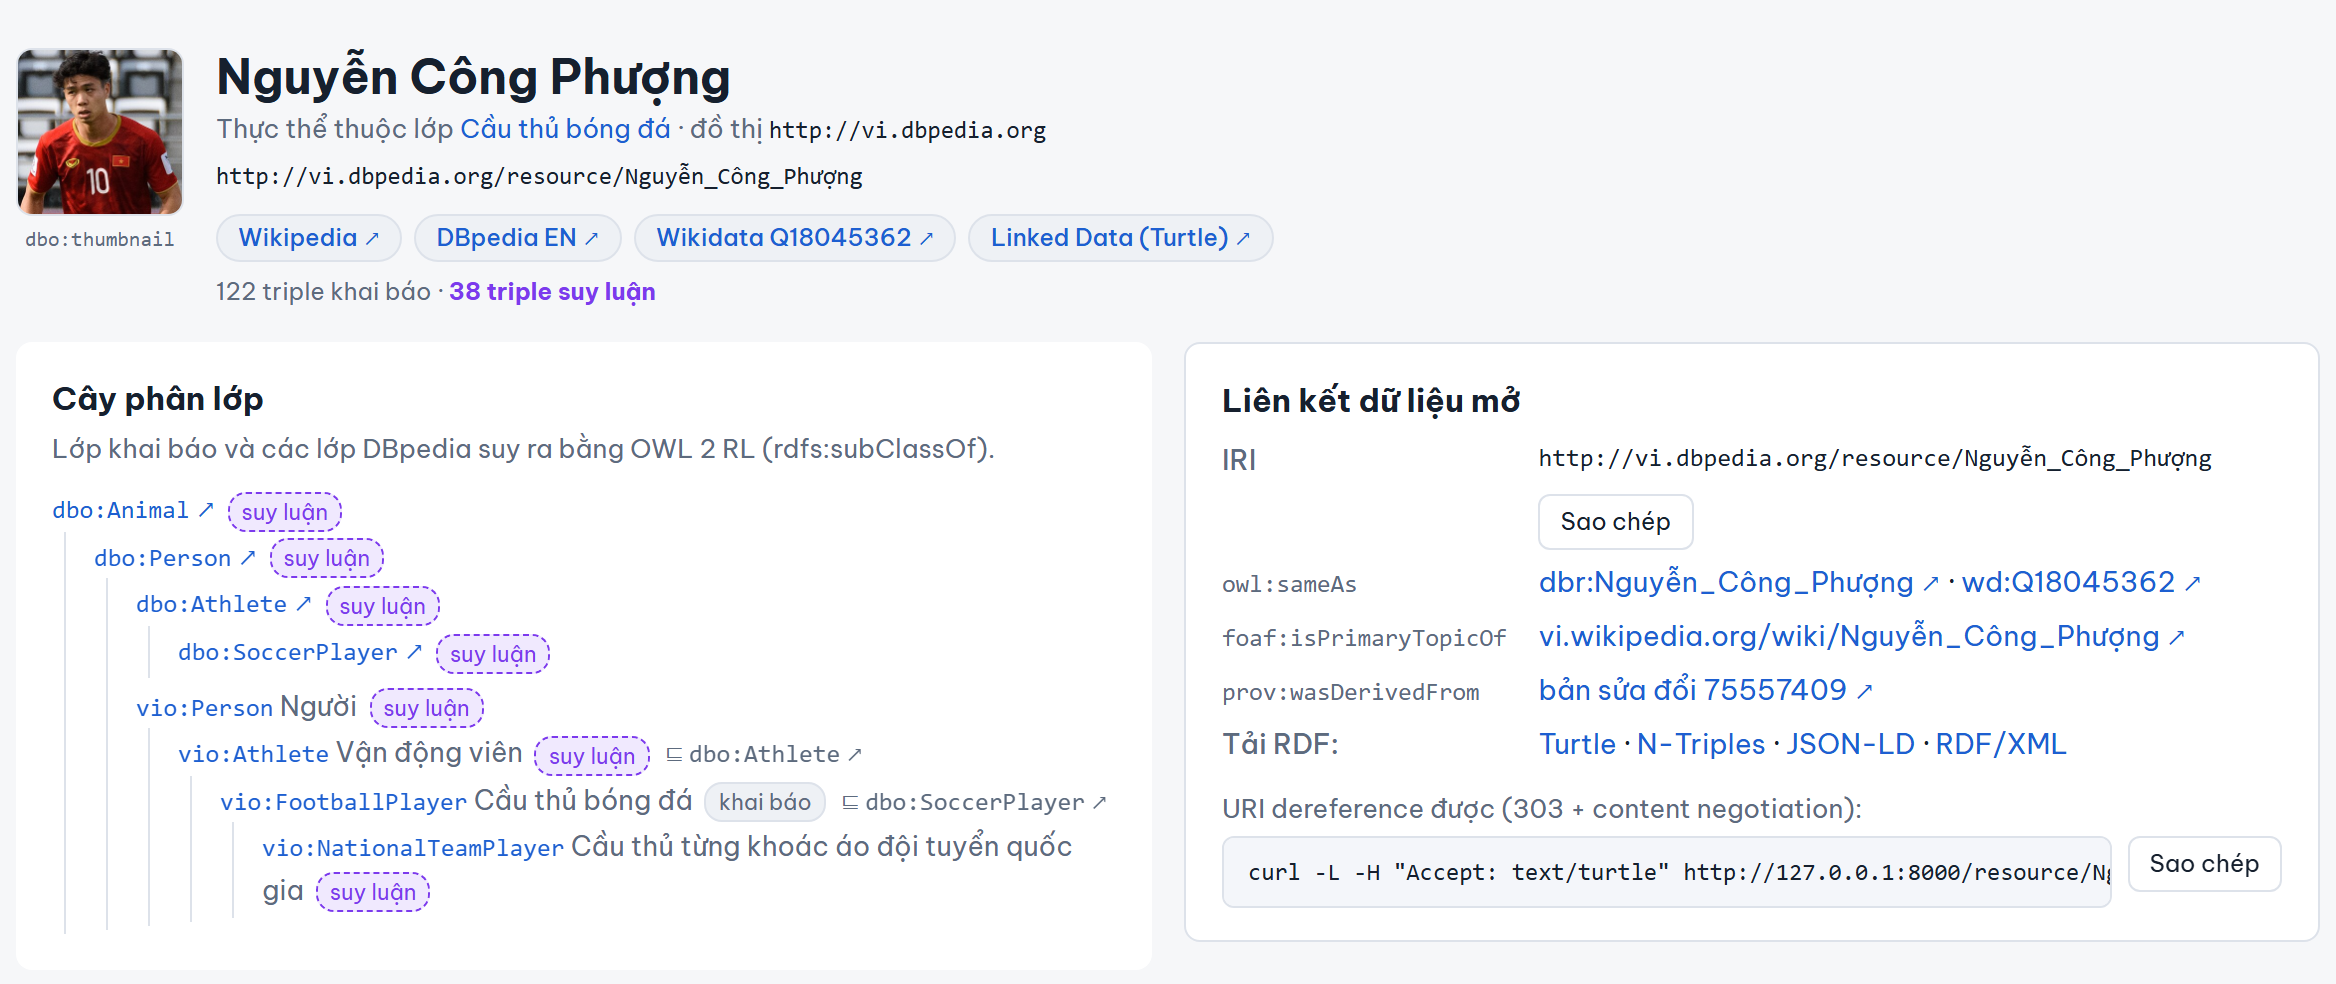
\includegraphics[width=\textwidth]{ui_entity.png}
\caption{Entity page of Nguyễn Công Phượng (abstract hidden): the asserted class and the named
graph, classes marked asserted (\emph{khai báo}) or inferred (\emph{suy luận}), and the
Linked Data card. Labels are in Vietnamese.}
\label{fig:ui}
\end{figure}

\begin{figure}[t]
\centering
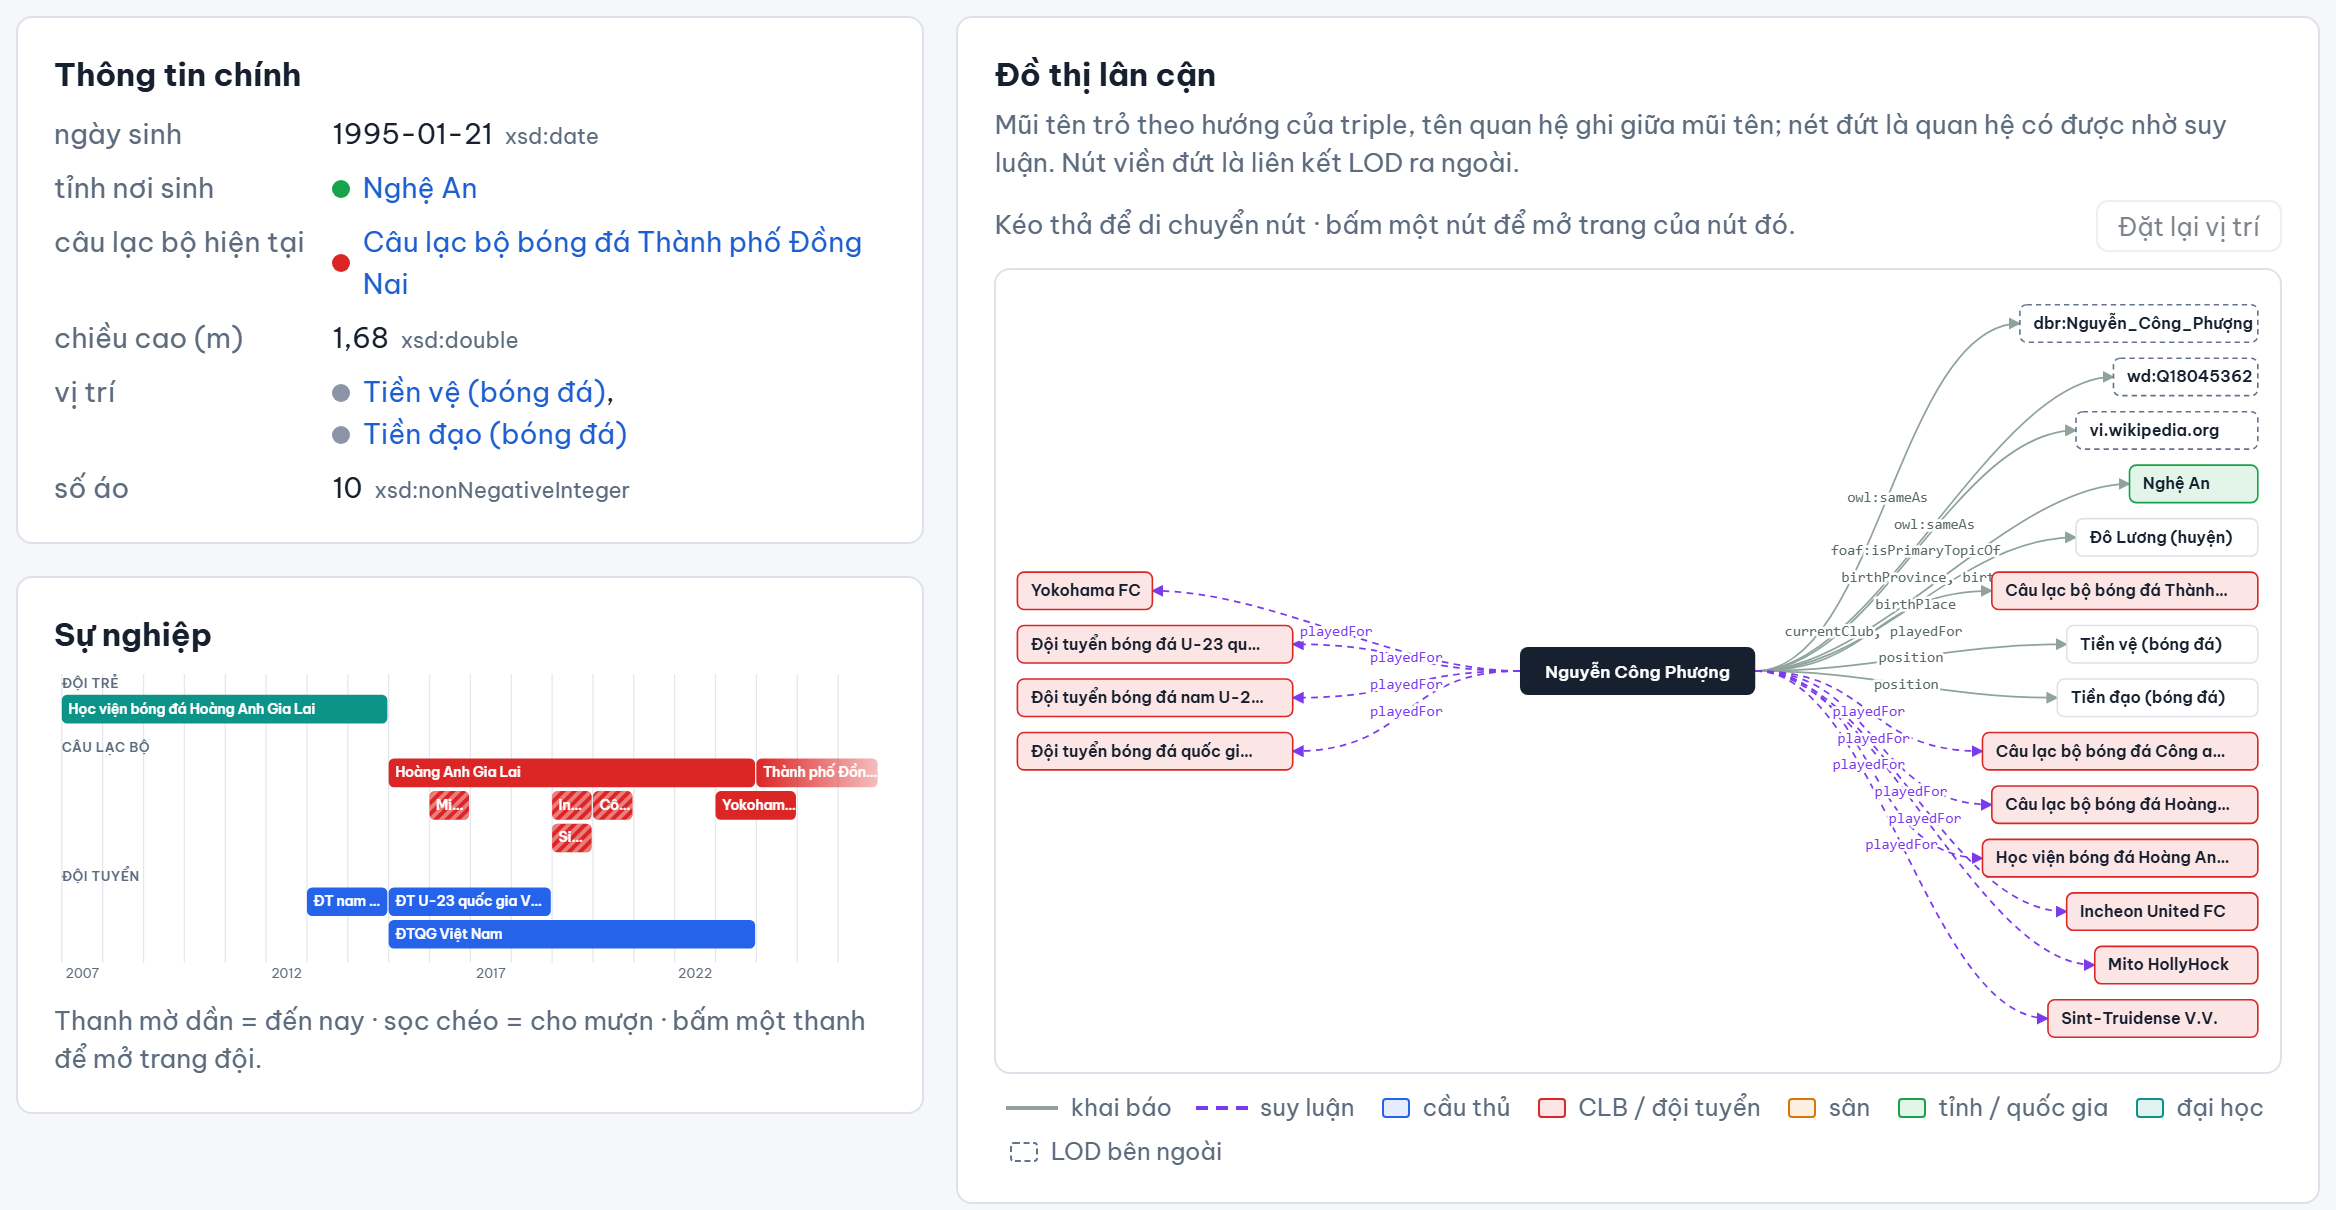
\includegraphics[width=\textwidth]{ui_entity_graph.png}
\caption{Lower part of the same page: key facts, career timeline and the draggable
neighbourhood graph, where the \term{playedFor} edges are dashed because they are inferred.}
\label{fig:ui-graph}
\end{figure}

\subsection{Natural-Language Question Answering}
\label{sec:qa}

\begin{figure}[t]
\centering
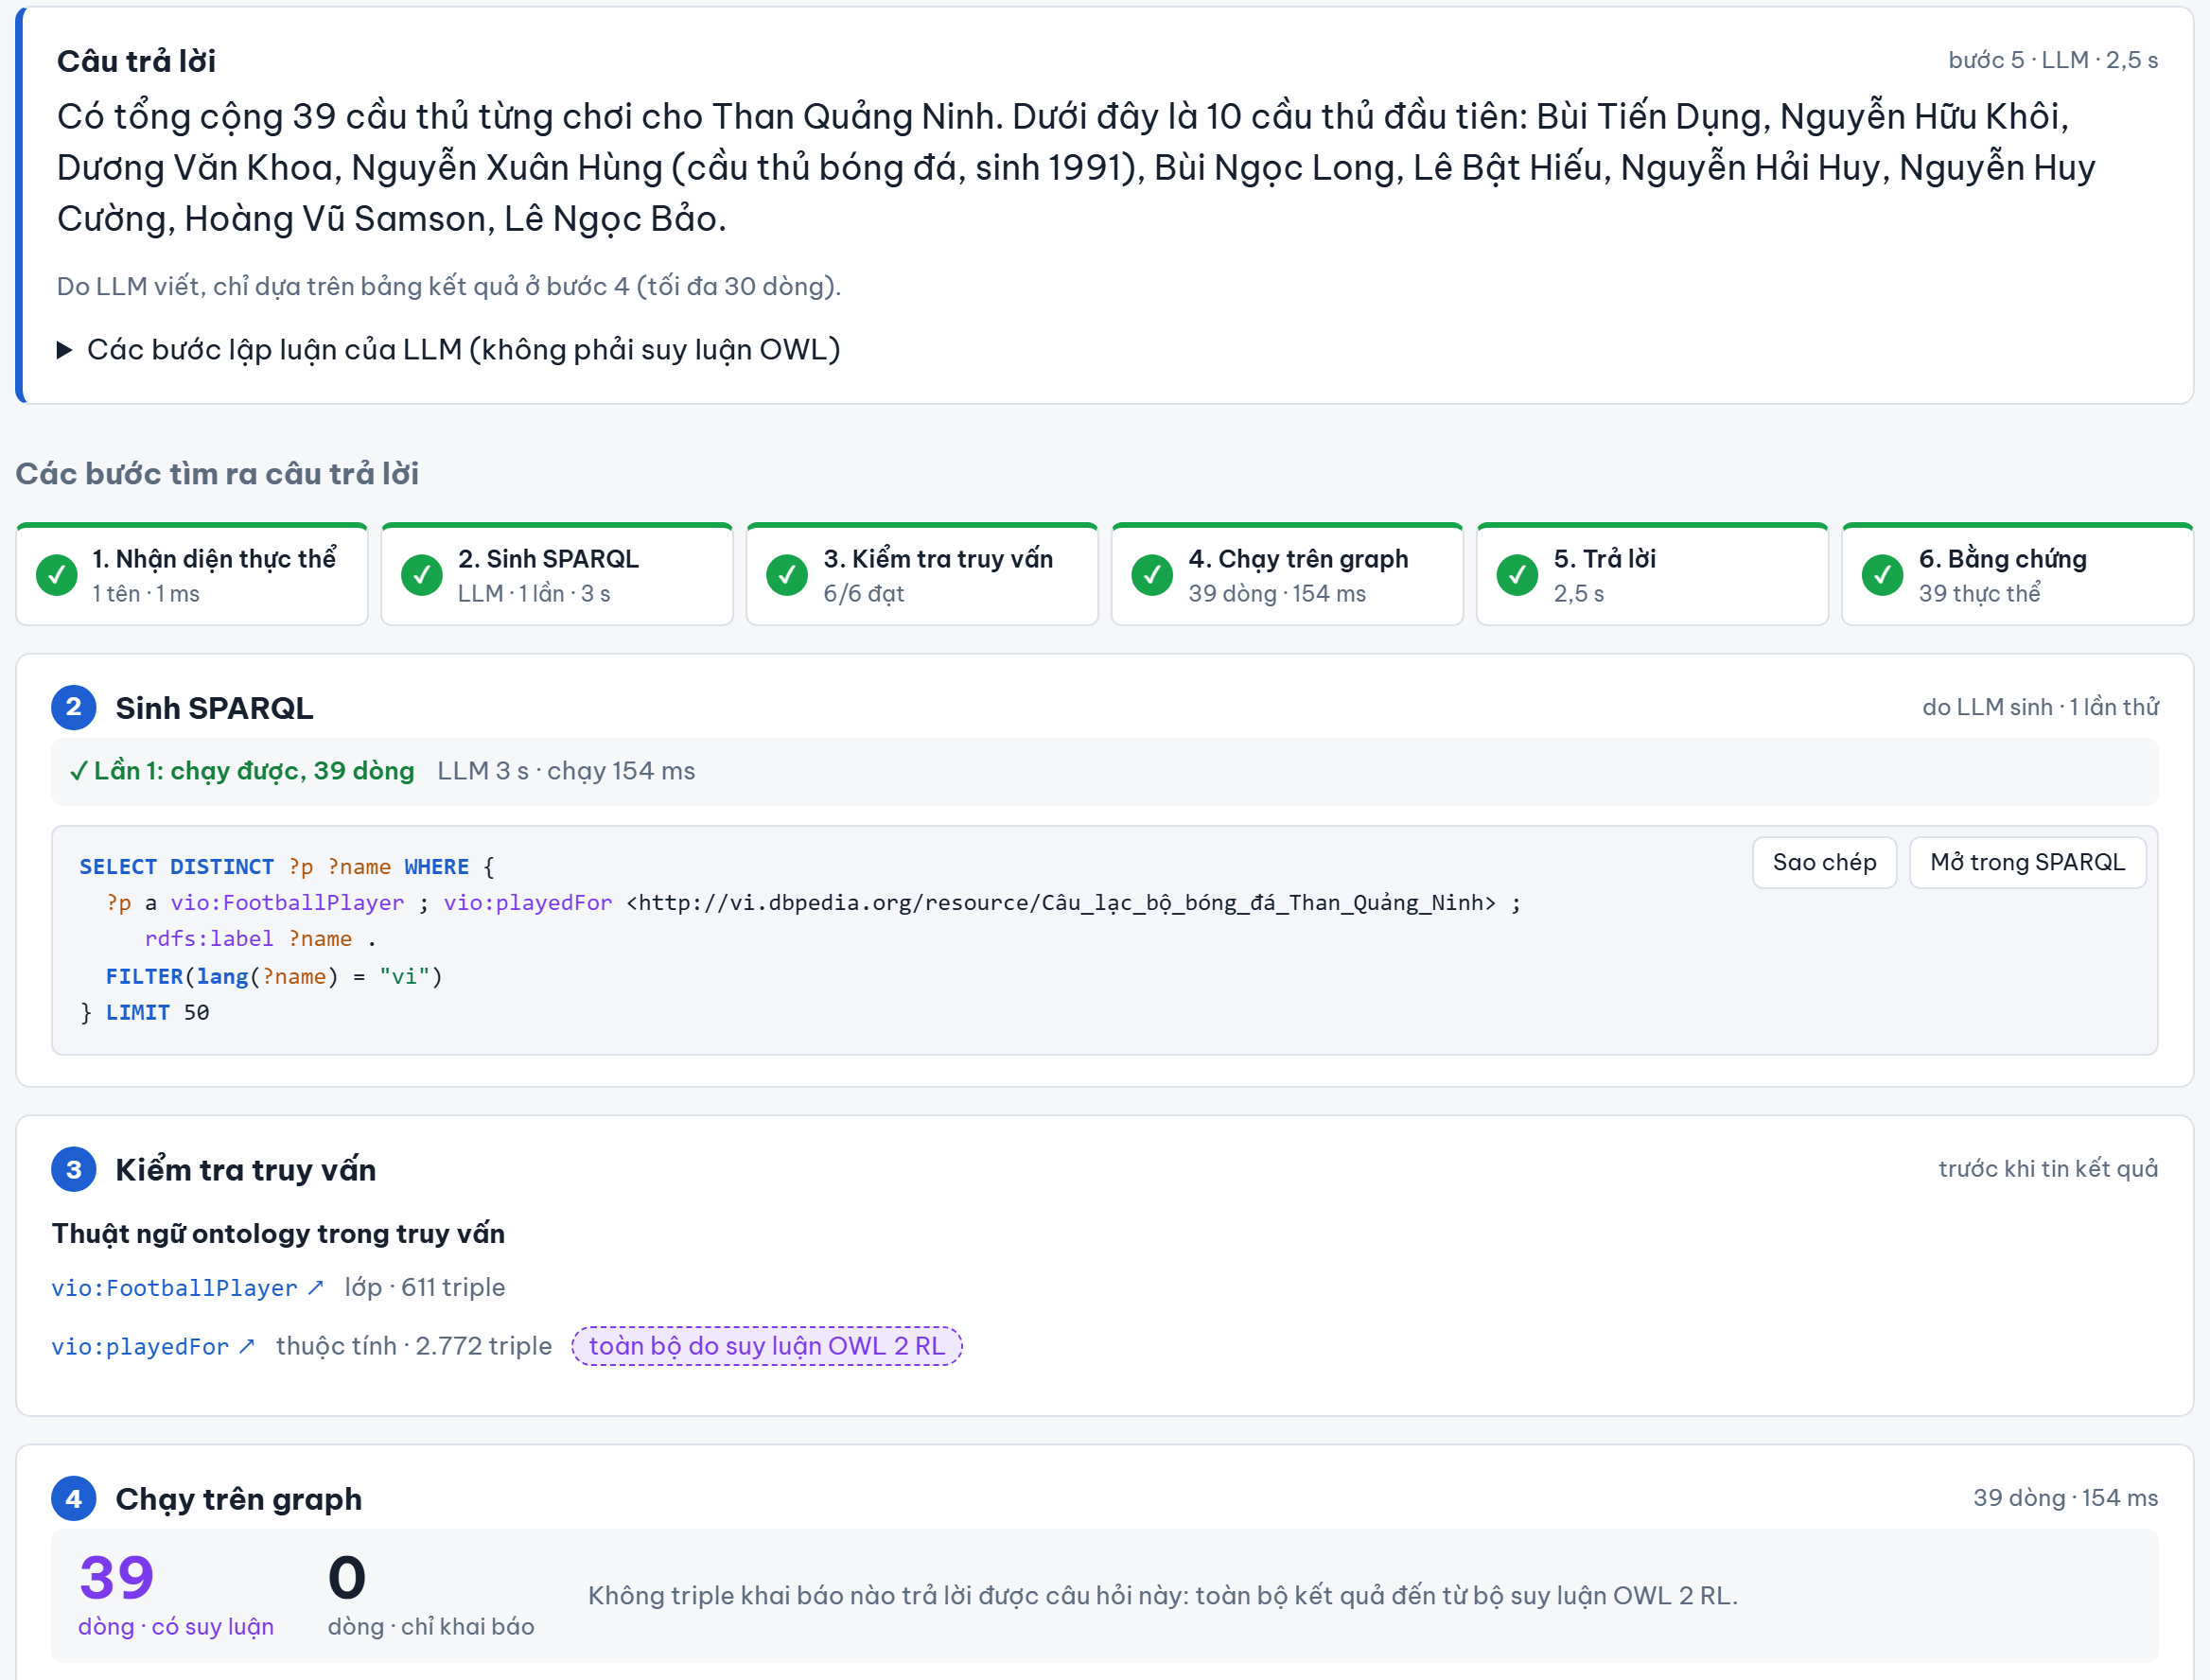
\includegraphics[width=\textwidth]{ui_ask.png}
\caption{Question answering with \term{gpt-4o} for ``which players have played for Than Quảng
Ninh?'': the answer, the progress of the six steps, the generated query, the ontology terms
with their inferred share, and 39 rows with reasoning against 0 without (step~1 and the
checks of step~3 hidden). Labels are in Vietnamese.}
\label{fig:qa}
\end{figure}

A language model writes a SPARQL query from a prompt with a schema summary,
rules (never guess IRIs, use the \term{playedFor} shortcut, skip former
provinces) and six example queries. A query that fails or returns no rows goes
back once with the error, and a second prompt answers from at most 30 rows;
any OpenAI-compatible API works.

\paragraph{Entity linking.} Step~1 needs no model. The labels (Vietnamese and
English) and redirect titles of the 1{,}176 entities of the main classes are
folded to lower case without diacritics and stored in two hash tables: whole
names, also without a bracketed qualifier, and the last two to four words of
each name, since Vietnamese names start with the type or the family name
(``Nguyễn Quang Hải''). Spans of the
question are looked up longest first; a matched word is not reused, spans of
generic words are skipped, and a name shared by up to six entities keeps them all.
Linking takes about 1\,ms.

The page shows the answer above the six steps behind it:
(1)~entity linking, whose IRIs are added to the prompt; (2)~each generation attempt, with feedback naming IRIs absent
from the graph or of the wrong class; (3)~checks of syntax, read-only
form, \term{FROM}, \term{SERVICE}, \term{LIMIT} and linked IRIs, with the
inferred share of each ontology term; (4)~execution with and without inferred
triples; (5)~the answer; and (6)~an evidence graph (Figure~\ref{fig:qa}).
The examples follow one performance rule: rdflib applies a \term{FILTER} only after
joining the whole group, so the lookup of an entity by name is written as a
subquery that runs first. For the career of Nguyễn Công Phượng this takes the
query from 10.7\,s to 0.27\,s.

\section{Evaluation}
\label{sec:evaluation}

All figures in this section are computed from the published dataset by
\term{report/report\_numbers.py}.

\subsection{Dataset and Coverage}
\label{sec:stats}

The dataset contains 131{,}543 triples: 88{,}898 asserted, 41{,}730 inferred,
859 in the ontology and 56 in the VoID description. They describe 990
entities, 3{,}382 career stations (527 youth, 1{,}966 club and 889
national-team stations), 1{,}154 categories and 1{,}274 redirects, for 8{,}624
distinct resource IRIs in total. 1{,}382 of these resources have a label but
no class. They are targets of links in infobox values, such as cities,
districts, people and competitions. Table~\ref{tab:coverage}
shows the coverage by class.

\begin{table}[t]
\centering
\caption{Entities by class, articles with an infobox, and entities linked to
English DBpedia.}
\label{tab:coverage}
\small
\begin{tabular}{@{}lrrr@{}}
\toprule
Class & Entities & With infobox & Linked to DBpedia \\
\midrule
Football players       & 611 & 602 & 508 \\
Football clubs         & 61  & 59  & 60 \\
National teams         & 10  & 5   & 10 \\
Stadiums               & 29  & 29  & 25 \\
Universities           & 168 & 159 & 89 \\
Provinces (34 current) & 110 & 101 & 84 \\
Country                & 1   & 1   & 1 \\
\midrule
Total                  & 990 & 956 (97\%) & 777 (78\%) \\
\bottomrule
\end{tabular}
\end{table}

Infobox coverage is high for every class except national teams, whose
Vietnamese articles often lack an infobox. Links to English DBpedia are
complete for clubs and national teams but cover about half of the
universities, many of which have no English article. Player properties are well
covered: position for 586 of 611 players, birth date for 572, height for 534,
birth province for 462 and current club for 442; 56 of 61 clubs have a home
ground and 142 of 168 universities a province. 129 of the 3{,}382 career
stations (3.8\%) have no \term{vio:team}, because the team is plain text in the
infobox or its link was rejected by the class filter.

\subsection{Effect of Reasoning}
\label{sec:reasoning-eval}

Table~\ref{tab:reasoning} compares queries on the asserted data alone with the
same queries on the published dataset. Of the 41{,}730 inferred triples,
18{,}341 are types and 23{,}389 are property values. Without reasoning, none of
the DBpedia classes or properties has an instance: the data uses only the
\term{vio:} vocabulary. After reasoning, a client that knows only DBpedia can
ask for \term{dbo:SoccerPlayer} or \term{dbo:team} and get answers. The 48
people who are not players (coaches, chairmen and rectors) receive
\term{dbo:Person} from the range of the property that links to them. The
property chain turns a two-step path through career stations into 2{,}772
direct \term{vio:playedFor} edges. The class counts of Table~\ref{tab:classes}
show the effect of the restrictions: 486 players become
\term{vio:NationalTeamPlayer}, and 154 clubs that are not seeds, such as
Mito HollyHock, become \term{vio:FootballClub} because they are the team of a
club station.

\begin{table}[t]
\centering
\caption{Answers to the same query on the asserted data alone and on the
published dataset (asserted plus inferred).}
\label{tab:reasoning}
\small
\begin{adjustbox}{max width=\textwidth}
\begin{tabular}{@{}lrrl@{}}
\toprule
Query pattern & Asserted & Published & Inferred through \\
\midrule
\term{?x a dbo:Person}           & 0 & 659     & subclass, \term{rdfs:range} \\
\term{?x a dbo:SoccerPlayer}     & 0 & 611     & \term{vio:FootballPlayer} $\sqsubseteq$ \term{dbo:SoccerPlayer} \\
\term{?x a dbo:Organisation}     & 0 & 410     & subclass \\
\term{?x a dbo:Place}            & 0 & 370     & subclass, \term{rdfs:range} \\
\term{?x vio:playedFor ?t}       & 0 & 2{,}772 & chain \term{careerStation} $\circ$ \term{team} \\
\term{?t vio:hasPlayer ?x}       & 0 & 2{,}772 & \term{owl:inverseOf} \\
\term{?x dbo:team ?t}            & 0 & 3{,}699 & sub-property \\
\term{?x dbo:birthPlace ?p}      & 0 & 802     & sub-property \\
\bottomrule
\end{tabular}
\end{adjustbox}
\end{table}

\subsection{Quality and Tests}
\label{sec:quality}

The eight checks of Table~\ref{tab:checks} report no error and no warning on
the last build. The test suite has 62 tests and passes in about 25\,s: 12
competency questions on the real data (Section~\ref{sec:cq}); 5 quality tests,
including the ontology conventions; 4 reasoning tests on small graphs; 6 parser
tests; 5 question-answering tests with a stubbed model; 19 tests of the Linked
Data routes, resource page and resource tree; and 11 tests of the endpoint and
terminal client, including the rejection of updates, \term{FROM} and
\term{SERVICE}. The interface adds 90 tests on the same data. Tests use lower
bounds instead of exact counts, so they keep passing after a new crawl.

\subsection{Links to English DBpedia}
\label{sec:links}

We sent every \term{dbr:} target to the public DBpedia SPARQL endpoint and
checked whether it describes an article, a redirect or nothing
(Table~\ref{tab:links}). 733 of the 777 links (94.3\%) point to an article,
which also confirms that DBpedia uses the same Unicode IRIs as we do. Twelve
point to a redirect (for example \term{dbr:Quảng\_Ninh}) and 32 to titles that
DBpedia does not contain, half of them clubs with recent titles such as
\term{dbr:Ho\_Chi\_Minh\_City\_FC\_(2025)}: our links come from today's English
Wikipedia, while DBpedia was extracted from an older snapshot.

\begin{table}[t]
\centering
\caption{\term{owl:sameAs} targets in English DBpedia, checked against
\term{dbpedia.org/sparql} on 7 October 2026.}
\label{tab:links}
\small
\begin{tabular}{@{}lrr@{}}
\toprule
Status of the \term{dbr:} target & Links & Share \\
\midrule
Article                                 & 733 & 94.3\% \\
Redirect (\term{dbo:wikiPageRedirects}) & 12  & 1.5\% \\
Not in DBpedia                          & 32  & 4.1\% \\
\midrule
Total                                   & 777 & 100\% \\
\bottomrule
\end{tabular}
\end{table}

\subsection{Competency Questions}
\label{sec:cq}

Table~\ref{tab:cq} lists competency questions that guided the ontology, with
the answers that the graph returns. Each question is a test in
\term{tests/test\_sparql.py}, and most need several hops or an inferred triple.

\begin{table}[t]
\centering
\caption{Competency questions and the answers returned by the graph.}
\label{tab:cq}
\small
\begin{tabularx}{\textwidth}{@{}>{\raggedright\arraybackslash}X>{\raggedright\arraybackslash}Xl@{}}
\toprule
Question & Answer & Relies on \\
\midrule
How many provinces and centrally governed cities are there now? & 34 (of 110 provinces, 76 are former) & \term{vio:FormerProvince} \\
Which unit succeeded the former province of Hà Tây? & Hà Nội & \term{vio:successor} \\
Which teams has Nguyễn Công Phượng played for? & 11 teams over 11 stations, 7 of them at clubs & property chain \\
Which provinces are home to the most players? & Nghệ An 58, Hà Nội 48, Thanh Hóa 42 & \term{vio:birthProvince} \\
How many universities are in Hà Nội? & 54 & \term{vio:province} \\
How many clubs have a home ground in a known province? & 44 & club $\rightarrow$ stadium $\rightarrow$ province \\
Which entity is meant by ``Công Phượng''? & Nguyễn Công Phượng & \term{dbo:wikiPageRedirects} \\
Which entities are DBpedia soccer players? & 611 & subclass reasoning \\
\bottomrule
\end{tabularx}
\end{table}

\subsection{Five-Star Assessment}
\label{sec:stars}

Table~\ref{tab:stars} assesses the dataset against the five-star
scheme~\cite{bernerslee2006linked}.

\begin{table}[t]
\centering
\caption{The dataset against the five-star scheme.}
\label{tab:stars}
\small
\begin{tabularx}{\textwidth}{@{}l>{\raggedright\arraybackslash}X@{}}
\toprule
Star & Evidence \\
\midrule
$\star$ open licence on the web & CC~BY-SA~4.0, declared in the VoID description and the ontology header; dumps published in a Git repository \\
$\star\star$ machine-readable & RDF triples, not text or tables \\
$\star\star\star$ open formats & Turtle and N-Triples dumps; each resource also as JSON-LD and RDF/XML; query results in the SPARQL JSON, XML and CSV formats \\
$\star\star\star\star$ URIs for things & an HTTP IRI for every entity, career station, category and redirect; dereferenced with 303 and content negotiation by the project server (Section~\ref{sec:deref}) \\
$\star\star\star\star\star$ linked & 777 \term{owl:sameAs} links to English DBpedia, 990 to Wikidata, described as VoID linksets; classes and properties aligned to \term{dbo:} \\
\bottomrule
\end{tabularx}
\end{table}

\section{Discussion}
\label{sec:discussion}

\paragraph{Design decisions.} Besides the selection through Wikidata and the
two-layer ontology (Sections~\ref{sec:collection} and~\ref{sec:ontology}),
inferred triples are \emph{materialised and stored separately}, so clients get
DBpedia types without a reasoner and the interface can mark what is inferred;
and \emph{one Python process with an in-memory rdflib graph} serves the
endpoint, the Linked Data routes and the interface. The 131 thousand triples
load in a few seconds; a triple store such as Virtuoso pays off when the data
grows.

\paragraph{Limitations.} The current system has six limitations.
\begin{itemize}
  \item \emph{Coverage.} 990 entities of one domain, not all of Vietnamese
        Wikipedia; each new class needs a seed query, ontology terms, an
        infobox mapping and a build function.
  \item \emph{Resolvable IRIs.} We do not control \term{vi.dbpedia.org}, so
        the IRIs dereference only through a running project server; a domain
        of our own or \term{w3id.org} would make them resolvable on the Web.
  \item \emph{Link drift.} 44 of the 777 English links do not reach a DBpedia
        article (Section~\ref{sec:links}); following
        \term{dbo:wikiPageRedirects} would fix twelve of them.
  \item \emph{Data gaps.} 129 career stations have no team IRI, 26
        universities have no province, and page links
        (\term{dbo:wikiPageWikiLink}) and \term{skos:broader} are not extracted.
  \item \emph{Serving.} The SPARQL endpoint has no query time limit, because
        rdflib cannot cancel a running query; a public deployment needs a
        stoppable process or a triple store that enforces a limit.
  \item \emph{Question answering.} Its quality depends on the language
        model and was not measured on a benchmark; the evidence graph is
        empty when the rows hold one end of each relation.
\end{itemize}

\section{Conclusion}
\label{sec:conclusion}

We built a DBpedia-style knowledge base for Vietnamese football, provinces and
universities that covers the five tasks of the assignment: a two-layer OWL
ontology aligned to the DBpedia Ontology; 990 entities selected through
Wikidata; 88{,}898 validated triples, which OWL~2~RL reasoning extends to
131{,}543; 777 links to English DBpedia (733 resolve) and 990 to Wikidata; and
a SPARQL endpoint, a terminal client, dereferenceable IRIs and a web interface
with question answering. Reasoning makes the data interoperable: it adds the
DBpedia types that clients expect and shortcut edges for multi-hop questions.

Future work follows from the limitations: query time limits or a triple store,
more classes (coaches, competitions) and page links, a link check against
DBpedia at every build, and a Vietnamese question-answering benchmark.


% =========================
% As in NeurIPS papers, the references follow the last section and may be set
% in \small (9pt).
\nocite{*}
{\small
\bibliographystyle{IEEEtran}
\bibliography{references}
}

\end{document}
